%%
%% This work consists of the files utfprpb.cls, utfprpb.tex, and
%% utfprpb-dados.tex.
%%
%% The Current Maintainer of this work is Vinicius Pegorini.
%% Updated by:
%% - Marco Aurélio Graciotto Silva;
%% - Rogério Aparecido Gonçalves;
%% - Luiz Arthur Feitosa dos Santos.
%%
%% This work consists of the files utfpr.cls, main.tex, and
%% variaveis.tex.
%% A brief description of this work is in readme.md.



%###################################################


% Luiz - pdfa: inclusão do pdfa
\PassOptionsToPackage{
	pdfa
}{hyperref}



%% Classe e opções de documento
\documentclass[%% Opções
%% -- Opções da classe memoir --
  12pt,%% Tamanho da fonte: 10pt, 11pt, 12pt, etc.
  a4paper,%% Tamanho do papel: a4paper (A4), letterpaper (carta), etc.
  % fleqn,%% Alinhamento das equações à esquerda (comente para alinhamento centralizado)
  % leqno,%% Numeração das equações no lado esquerdo (comente para lado direito)
  oneside,%% Impressão dos elementos textuais e pós-textuais: oneside (anverso) ou twoside (anverso e verso, se mais de 100 p.)
  openright,%% Impressão da primeira página dos capítulos: openright (anverso), openleft (verso) ou openany (anverso e verso)
%% -- Opções da classe abntex2 --
  sumario = abnt-6027-2012,%% Formatação do sumário: tradicional (estilo tradicional) ou abnt-6027-2012 (norma ABNT 6027-2012)
  chapter = TITLE,%% Títulos de capítulos em maiúsculas (comente para desabilitar)
  % luiz - comentar section para ser minusculo
  %section = TITLE,%% Títulos de seções secundárias em maiúsculas (comente para desabilitar)
  % subsection = TITLE,%% Títulos de seções terciárias em maiúsculas (comente para desabilitar)
  % subsubsection = TITLE,%% Títulos de seções quartenárias em maiúsculas (comente para desabilitar),
%% -- Opções da classe utfprpgtex --
  pretextualoneside,%% Impressão dos elementos pré  -textuais: pretextualoneside (anverso) ou pretextualtwoside (anverso e verso)
  fontetimes,%% Fonte do texto: fontetimes (times), fontearial (arial) ou fontecourier (courier)
  % vinculoscoloridos,%% Cores nos vínculos (citações, arquivos, links, url, etc.) (comente para desabilitar)
  semrecuonosumario,%% Remoção do recuo dos itens no sumário (comente para adição do recuo, se estilo tradicional)
  usemakeindex,%% Compilação de glossários e índices utilizando makeindex (comente para desabilitar)
  % legendascentralizadas,%% Alinhamento das legendas centralizado (comente para alinhamento à esquerda)
  %aprovacaoestiloppg,%% Folha de aprovação do programa de pós-graduação no estilo do PPG (comente para estilo padrão)
  pardeassinaturas,%% Assinaturas na folha de aprovação em até duas colunas (comente para em uma única coluna)
  % linhasdeassinaturas,%% Linhas de assinaturas na folha de aprovação (comente para remover as linhas)
%% -- Opções do pacote babel --
  english,%% Idioma adicional para hifenização
  french,%% Idioma adicional para hifenização
  spanish,%% Idioma adicional para hifenização
  brazil,%% Idioma principal do documento (último da lista)
]{utfpr}%% Classe utfpr


% Luiz: pdfa: necessário para criar pdfa
\usepackage[a-3b,mathxmp]{pdfx}[2018/12/22] % você pode escolher entre a-1b, a-2b, a-3b - o template ainda não suporta o a-Xa de 
%%%% configuracoes.tex, 2022/05/02, 2.4a

%% ####################################################
%%
%% >> Atenção - Leia isso antes de usar esse template<< 
%%
%% Esse template foi desenvolvido por professores,  com a intenção de ajudar os alunos com as entregas na biblioteca. Não há uma equipe especializada e dedicada mantendo tal template, mas sim professores trabalhando além das suas funções básicas, que são: ensino, pesquisa e extensão.
%
%% Também os mantenedores deste template não são especializados em LaTeX, muito menos em normas da ABNT. Todos que contribuíram com o template fizeram isso visando deixá-lo o mais próximo possível das normas da ABNT e das regras, anseios e expectativas da biblioteca da UTFPR. É muito importante entender que os desenvolvedores do template não têm relação direta com a biblioteca ou com a ABNT. Ou seja, não são os desenvolvedores do template que ditam as regras e normas dos textos que devem ser entregues à biblioteca.

%%É válido informar também, que como não há uma equipe dedicada e especializada, o tempo para colaborar com o template é curto. Desta forma, pode ser que não sejam empregadas as melhores técnicas, métodos e ferramentas para o desenvolvimento do template. Também pode acontecer do template não atender completamente todos os anseios e exigências da ABNT e da biblioteca, pois por exemplo, muitas regras de redação possuem questões interpretativas. Assim, o template sempre estará em contínua evolução e seria extremamente interessante que as pessoas (alunos,  professores,  técnicos e entusiastas) colaborarem com a evolução do template. Toda ajuda será bem vinda! Isso pode ser feito enviando e-mail para os desenvolvedores, desta forma, assim que possível esses vão tentar melhorar o template.

%%O template é apenas mais uma ferramenta para o desenvolvimento de trabalhos para a biblioteca. Todavia, podem existir outros templates LaTeX. Assim como há templates em outros formatos, que não o LaTeX. O mais importante é que qualquer pessoa, utilizando a princípio qualquer ferramenta, pode desenvolver textos que atendem os requisitos da biblioteca apenas estudando, interpretando e seguindo as regras da UTFPR e da ABNT, que estão disponíveis na página Web da instituição. O template é só um facilitador.

%%Por fim,  é necessário entender que infelizmente o ambiente LaTeX pode ser complexo e gerar resultados distintos dependendo do: sistema operacional,  pacotes LaTeX utilizados,  configurações alteradas, editor utilizado, a forma que está sendo redigida textos, figuras,  etc. Assim não há como garantir que o resultado final será o esperado.  Dito tudo isso,  >>UTILIZE ESSE TEMPLATE POR SUA CONTA E RISCO<<. Os desenvolvedores e colaboradores deste template não se responsabilizam pelo resultado do uso deste template e se eximem de qualquer responsabilidade.

%###################################################

%% Pacotes carregados nas classes:
%%   memoir: abstract, appendix, array, booktabs, ccaption, chngcntr, chngpage, dcolumn, delarray, enumerate, epigraph, framed,
%%           ifmtarg, ifpdf, index, makeidx, moreverb, needspace, newfile, nextpage, parskip, patchcmd, setspace, shortvrb, showidx,
%%           tabularx, titleref, titling, tocbibind, tocloft, verbatim, verse.
%%   memoir (similares): crop, fancyhdr, geometry, sidecap, subfigure, titlesec.
%%   abntex2: babel, bookmark, calc, enumitem, ifthen, hyperref, textcase.
%%   utfprpgtex: abntex2cite, ae, algorithmic, amsmath, backref, breakurl, caption, cmap, color, eepic, epic, epsfig, etoolbox,
%%               fancyhdr, fix-cm, fontenc, glossaries, graphics, graphicx, helvet, hyphenat, indentfirst, inputenc, lastpage,
%%               morewrites, nomencl, sfmath, sistyle, substr, times, xtab.


%% Pacotes adicionais (\usepackage[options]{package})
\usepackage{bigdelim, booktabs, colortbl, longtable, multirow}%% Ferramentas para tabelas
\usepackage{amssymb, amstext, amsthm, icomma}%% Ferramentas para linguagem matemática
\usepackage{pifont, textcomp, wasysym}%% Símbolos de texto
\usepackage{lipsum}				% para geração de dummy text
\usepackage{subfig}             % para adicionar figuras lado a lado no texto                    
\usepackage{pdfpages}           % para adicionar documentos pdf ao trabalho
\usepackage{xspace}
\usepackage{xcolor}


% luiz: primeira letra maiúscula
% solução 1
%\usepackage{stringstrings}
%\newcommand{\firstcap}[1]{\caselower[e]{#1}\capitalize{\thestring}}

% solução 2 - não usei essa
% \usepackage[utf8]{inputenc}
% \usepackage{datatool-base}
% \usepackage{mfirstuc}

% Formatação do título da seção - primeira letra caixa alta e o resto em caixa baixa.
% \usepackage[explicit]{titlesec}
% \usepackage{lipsum}
% \titleformat{\section}{\normalfont}{\thesection}{1em}{\textbf{\firstcap{#1}}} % funciona mas apenas para o título da seção e não para o sumário (a configuração do sumário está mais para baixo

% luiz: define o underline colorido.
% https://github.com/abntex/abntex2-contrib/blob/master/customizacoes/pucminas/abntex2-pucminas.sty
% acabei não usando o black e o coloruline da solução do link

\usepackage[normalem]{ulem} % para o underline colorido na seção quaternária
\renewcommand*{\cftsubsubsectionfont}{\normalfont\uline} % underline no sumário
\setsubsubsecheadstyle{\ABNTEXsubsubsectionfont\ABNTEXsubsubsectionfontsize\ABNTEXsubsubsectionupperifneeded\uline} %underline no título da subsubsection

% luiz: bibliografia - opções

%% Comandos personalizados (\newcommand{name}[num]{definition})
\newcommand{\cpp}{\texttt{C$++$}}%% C++
\newcommand{\latex}{\LaTeX\xspace}%% LaTeX
\newcommand{\ds}{\displaystyle}%% Tamanho normal das equações
\newcommand{\bsym}[1]{\boldsymbol{#1}}%% Texto no modo matemático em negrito
\newcommand{\mr}[1]{\mathrm{#1}}%% Texto no modo matemático normal (não itálico)
\newcommand{\der}{\mr{d}}%% Operador diferencial
\newcommand{\deri}[2]{\frac{\der #1}{\der #2}}%% Derivada ordinária
\newcommand{\derip}[2]{\frac{\partial #1}{\partial #2}}%% Derivada parcial
\newcommand{\pare}[1]{\left( #1 \right)}%% Parênteses
\newcommand{\colc}[1]{\left[ #1 \right]}%% Colchetes
\newcommand{\chav}[1]{\left\lbrace #1 \right\rbrace}%% Chaves
\newcommand{\sen}{\operatorname{sen}}%% Operador seno
\newcommand{\senh}{\operatorname{senh}}%% Operador seno hiperbólico
\newcommand{\tg}{\operatorname{tg}}%% Operador tangente
\newcommand{\tgh}{\operatorname{tgh}}%% Operador tangente hiperbólico
\newcommand{\seqref}[1]{Equação~\eqref{#1}}%% Referência de uma única equação
\newcommand{\meqref}[1]{Equações~\eqref{#1}}%% Referência de múltiplas equações
\newcommand{\citep}[1]{\cite{#1}}%% Atalho para citação implícita
\newcommand{\citet}[1]{\citeonline{#1}}%% Atalho para citação explícita
\newcommand{\citepa}[1]{(\citeauthor{#1})}%% Atalho para citação implícita (somente autor)
\newcommand{\citeta}[1]{\citeauthoronline{#1}}%% Atalho para citação explícita (somente autor)
\newcommand{\citepy}[1]{(\citeyear{#1})}%% Atalho para citação implícita (somente ano)
\newcommand{\citety}[1]{\citeyear{#1}}%% Atalho para citação explícita (somente ano)

\newcommand{\fonteTexto}[1]{\renewcommand{\familydefault}{#1}}

% Define o caminho das figuras
\graphicspath{{figuras/}}

% Define a fonte ara helvet que é uma fonte similar à Arial, se for usar a Arial tem que mudar o compilador para XeLaTex, mas ai tem que arrumar os erros: https://latex.org/forum/viewtopic.php?t=25998
%\usepackage{helvet}
%\renewcommand{\familydefault}{\sfdefault}
%\usepackage{times} % para fonte time new roman
%\usepackage{pslatex} % ou essa aqui...

%\usepackage{titlesec}

%% Configuração de glossário
% \usepackage[portuguese]{nomencl}
% \usepackage[nogroupskip,nonumberlist,nopostdot,nohypertypes={acronym}]{glossaries}
% \makenoidxglossaries
\usepackage{glossaries}
\makeglossaries

% para siglas em português
\newcommand{\siglaPt}[2]
{
 \newglossaryentry{#1}{
  name=#1,
  description={#2},
  first={#2 (#1)},
  long={#2}
 }  
}

% para siglas de língua estrangeira, nessas a descrição longa fica em itálico.
\newcommand{\siglaIt}[2]
{
 \newglossaryentry{#1}{
  name=#1,
  description={\textit{#2}},
  first={\textit{#2} ({#1})},
  long={\textit{#2}}
 }  
}

%% luiz - para fazer os avisos
\usepackage{tcolorbox}

% use para criar caixas de avisos, pode ser utilizado para fazer anotações de tarefas indicadas pelo orientador/banca.
% \caixa{Atenção}{texto...}
\newcommand{\caixa}[2]{
\begin{tcolorbox}[colback=red!5!white,colframe=red!45!white, title = #1, fonttitle=\bfseries]
#2
\end{tcolorbox}
}

% Luiz - Linhas órfãs e viúvas
\widowpenalty=10000
\clubpenalty=10000

% Luiz - Caption do tamanho da Tabela
%\usepackage[width=1\textwidth]{caption}

% Luiz - configurar a margem dos itens
\setlength{\leftmargini}{1.5cm}
\setlength{\leftmarginii}{1.5cm}



%% Arquivo de dados do modelo de documento LaTeX para produção de trabalhos acadêmicos da UTFPR
%%%% variaveis.tex, 2022/05/02, 2.4a
%%%% Copyright (C) 2020 Vinicius Pegorini (vinicius@utfpr.edu.br)
%%
%% This work may be distributed and/or modified under the conditions of the
%% LaTeX Project Public License, either version 1.3 of this license or (at your
%% option) any later version.
%% The latest version of this license is in
%%   http://www.latex-project.org/lppl.txt
%% and version 1.3 or later is part of all distributions of LaTeX version
%% 2005/12/01 or later.
%%
%% This work has the LPPL maintenance status `maintained'.
%%
%% The Current Maintainer of this work is Vinicius Pegorini.
%% Updated by:
%% - Marco Aurélio Graciotto Silva;
%% - Rogério Aparecido Gonçalves;
%% - Luiz Arthur Feitosa dos Santos.
%%
%% This work consists of the files utfpr.cls, main.tex, and
%% variaveis.tex.
%%
%% A brief description of this work is in readme.txt.

%% ####################################################
%%
%% >> Atenção - Leia isso antes de usar esse template<< 
%%
%% Esse template foi desenvolvido por professores,  com a intenção de ajudar os alunos com as entregas na biblioteca. Não há uma equipe especializada e dedicada mantendo tal template, mas sim professores trabalhando além das suas funções básicas, que são: ensino, pesquisa e extensão.
%
%% Também os mantenedores deste template não são especializados em LaTeX, muito menos em normas da ABNT. Todos que contribuíram com o template fizeram isso visando deixá-lo o mais próximo possível das normas da ABNT e das regras, anseios e expectativas da biblioteca da UTFPR. É muito importante entender que os desenvolvedores do template não têm relação direta com a biblioteca ou com a ABNT. Ou seja, não são os desenvolvedores do template que ditam as regras e normas dos textos que devem ser entregues à biblioteca.

%%É válido informar também, que como não há uma equipe dedicada e especializada, o tempo para colaborar com o template é curto. Desta forma, pode ser que não sejam empregadas as melhores técnicas, métodos e ferramentas para o desenvolvimento do template. Também pode acontecer do template não atender completamente todos os anseios e exigências da ABNT e da biblioteca, pois por exemplo, muitas regras de redação possuem questões interpretativas. Assim, o template sempre estará em contínua evolução e seria extremamente interessante que as pessoas (alunos,  professores,  técnicos e entusiastas) colaborarem com a evolução do template. Toda ajuda será bem vinda! Isso pode ser feito enviando e-mail para os desenvolvedores, desta forma, assim que possível esses vão tentar melhorar o template.

%%O template é apenas mais uma ferramenta para o desenvolvimento de trabalhos para a biblioteca. Todavia, podem existir outros templates LaTeX. Assim como há templates em outros formatos, que não o LaTeX. O mais importante é que qualquer pessoa, utilizando a princípio qualquer ferramenta, pode desenvolver textos que atendem os requisitos da biblioteca apenas estudando, interpretando e seguindo as regras da UTFPR e da ABNT, que estão disponíveis na página Web da instituição. O template é só um facilitador.

%%Por fim,  é necessário entender que infelizmente o ambiente LaTeX pode ser complexo e gerar resultados distintos dependendo do: sistema operacional,  pacotes LaTeX utilizados,  configurações alteradas, editor utilizado, a forma que está sendo redigida textos, figuras,  etc. Assim não há como garantir que o resultado final será o esperado.  Dito tudo isso,  >>UTILIZE ESSE TEMPLATE POR SUA CONTA E RISCO<<. Os desenvolvedores e colaboradores deste template não se responsabilizam pelo resultado do uso deste template e se eximem de qualquer responsabilidade.

%###################################################

%% Documento
%% Luiz: Define a fonte do texto da monografia
\fonteTexto{\sfdefault} % utilize \rmdefault para Times New Roman ou \sfdefault para Arial
\TipoDeDocumento{Trabalho de Conclusão de Curso de Graduação}%% Tipo de documento: "Tese", "Dissertação" ou "Trabalho de Conclusão de Curso de Graduação", "Estágio Supervisionado"
\NivelDeFormacao{Bacharelado}%% Nível de formação: "Doutorado", "Mestrado", "Bacharelado" ou "Tecnólogo" - ATENÇÃO, isso será utilizado para alterar a formatação do trabalho, pois pode haver formatações distintas dependendo o nível/tipo de trabalho.


%% luiz
% Template LaTex criado pelo Departamento Acadêmico de Computação (DACOM)
% da Universidade Tecnológica Federal do Paraná - Campus Campo Mourão (UTFPR-CM)
% Criado e alterado pelos professores:
% - Marco Aurélio Graciotto Silva
% - Rogério Aparecido Gonçalvez
% - Luiz Arthur Feitosa dos Santos
% Esse template utiliza a licença CC BY:
% Esta licença permite que outros distribuam, remixem, adaptem e criem a partir deste trabalho, mesmo para fins comerciais, desde que atribuam o devido crédito pela criação original.
% https://creativecommons.org/licenses/by/4.0/deed.pt_BR

% Dados do curso. Caso seja BCC:
\program{\textcolor{red}{Nome do Curso / Programa}}
\programen{Undergradute Program in Computer Science}
\degree{\textcolor{red}{Bacharel / Licenciado / Tecnólogo / Mestre / Doutor}}
\degreearea{}
% Caso seja TSI:
% \program{Curso Superior de Tecnologia em Sistemas para Internet}
% \programen{Undergradute Program in Tecnology for Internet Systems}
% \degree{Tecnólogo}
% \degreearea{Tecnologia em Sistemas para Internet}


% Dados da disciplina. Escolha uma das opções e a descomente:
% TCC1:
%\goal{Proposta de Trabalho de Conclusão de Curso de Graduação}
%\course{Trabalho de Conclusão de Curso 1}
% TCC2:
\colorlet{RED}{red}

 \goal{\textcolor{red}{Trabalho de Conclusão de Curso de Graduação / Dissertação / Tese} apresentado (a)}
 \course{Trabalho de Conclusão de Curso 2}


% Dados do TCC (precisa alterar)
\author{NOME COMPLETO E POR EXTENSO DO(A) AUTOR(A)}  % Seu nome
\authorbib{Silva, João da} % Seu nome para referência bibliográfica (Sobrenome, Nome)
\title{O TÍTULO DEVE SER CLARO E PRECISO: SUBTÍTULO (SE HOUVER) DEVE SER PRECEDIDO DE DOIS PONTOS CONFIRMANDO SUA VINCULAÇÃO AO TÍTULO 
} % Título do trabalho

%Comentar esta linha na versão final
\titleNote{O título do trabalho constante na capa, na folha de rosto e na folha de aprovação deve ser idêntico ao registrado no Sistema Acadêmico.\\ (todo o texto destacado em vermelho deverá ser substituído e/ou excluído para a versão final).}

%Descomentar essa linha na versão final
%\titleNote{}

%Comentar a linha abaixo na versão final
\titleApNote{Este é um modelo de folha de aprovação destinado para os TCCs e TCCEs. Para dissertações e teses, a folha de aprovação deverá ser gerada pelo Sistema Acadêmico e inserida na versão final como texto (não inserir como imagem)}

%Descomentar a linha abaixo na versão final
%\titleApNote{}

\titleFA{TÍTULO DO TRABALHO: SUBTÍTULO (SE HOUVER) PRECEDIDO DE DOIS PONTOS}

\titleen{Título traduzido em língua inglesa título traduzido em língua inglesa título traduzido em língua inglesa título traduzido em língua inglesa} % Título traduzido para inglês
\advisor{Nome completo e por extenso conforme Currículo Lattes.} % Nome do orientador. Lembre-se de prefixar com "Prof. Dr.", "Profª. Drª.", "Prof. Me." ou "Profª. Me."}
% Se não houver corientador, comente a linha a baixo
\coadvisor{Nome completo e por extenso conforme Currículo Lattes.} % Nome do coorientador, caso exista. Caso não exista, comente a linha.
\depositshortdate{ANO DA ENTREGA} % Ano em que depositou este documento
\approvaldate{dia / mês por extenso / ano}

% Dados do curso que não precisam de alteração
\university{Universidade Tecnológica Federal do Paraná}
\universityen{Federal University of Technology -- Paraná}
\universitycampus{Campus Campo Mourão}
\universityunit{Departamento Acadêmico de Computação}
\address{CIDADE}
\addressen{Campus Cornélio Procópio, PR, Brazil}
\documenttype{Monografia}
\documenttypeen{Monograph}
\degreetype{Graduação}

\evalboardmember{Nome completo e por extenso do Membro 1 (de acordo com o Currículo Lattes)
}{Titulação (Especialização, Mestrado, Doutorado)}{Nome completo e por extenso da instituição a qual possui vínculo}
\evalboardmember{Nome completo e por extenso do Membro 2 (de acordo com o Currículo Lattes)
}{Titulação (Especialização, Mestrado, Doutorado)}{Nome completo e por extenso da instituição a qual possui vínculo}
\evalboardmember{Nome completo e por extenso do Membro 3 (de acordo com o Currículo Lattes)
}{Título (Titulação (Especialização, Mestrado, Doutorado)}{Nome completo e por extenso da instituição a qual possui vínculo}
%\evalboardmember{Nome completo e por extenso do Membro 4}{Título (especialização, mestrado, doutorado}{Nome completo e por extenso da instituição a qual possui vínculo}

%% Palavras-chave e keywords
%% ATENÇÃO - você deve indicar a quantidade de palavras chaves para o template LaTeX utilizar o pontuação correta!
\NumeroDePalavrasChave{4}%% Número de palavras-chave (máximo 5)
%% Atenção - por enquanto o template não está suportando acentos normais na palavra chave, por isso caso a palavra tenha acento, você deve utilizar o estilo antigo do LaTeX, sendo os acentos: á - \'a  é - \'e   â - \^a  ê - \^e  à - \`a  ä - \"a  ç - \c{c}
\PalavraChaveA{palavra 1}%% Palavra-chave A
\PalavraChaveB{palavra 2}%% Palavra-chave B
\PalavraChaveC{palavra 3}%% Palavra-chave C
\PalavraChaveD{palavra 4}%% Palavra-chave D
%\PalavraChaveE{Palavra-chave 5}%% Palavra-chave E
%% Exemplo de como utilizar acentos na Palavra-chave:
% \PalavraChaveA{ol\'a}%% Olá
%\PalavraChaveB{voc\^e}%% você
%\PalavraChaveC{\`a}%% à
%\PalavraChaveD{a\c{c}\~ao}%% ação
%\PalavraChaveE{arg\"uir}%% argüir


%% ATENÇÃO - você deve indicar a quantidade de keywords para o template LaTeX utilizar o pontuação correta!
\NumeroDeKeywords{4}%% Número de keywords (máximo 5)
\KeywordA{word 1}%% Keyword A
\KeywordB{word 2}%% Keyword B
\KeywordC{word 3}%% Keyword C
\KeywordD{word 4}%% Keyword D
%\KeywordE{Keyword 5}%% Keyword E


% É obrigatório o uso de uma licença Creative Commons (CC) nos trabalhos de TCC pelos cursos ligados a DACOM da UTFPR-CM.
% Veja: http://portal.utfpr.edu.br/biblioteca/trabalhos-academicos/docentes/procedimento-de-entrega-graduacao

% Sendo assim, escolha com o seu orientador uma das licenças CC a seguir: 

% CC BY: Esta licença permite que outros distribuam, remixem, adaptem e criem a partir deste trabalho, mesmo para fins comerciais, desde que atribuam o devido crédito pela criação original. Essa é a menos restritiva.
\licenca{ccby}

% CC BY CA: Esta licença permite que outros remixem, adaptem e criem a partir deste trabalho, mesmo para fins comerciais, desde que atribuam o devido crédito e que licenciem as novas criações sob termos idênticos.
%\licenca{ccbysa}

% CC BY ND: Esta licença permite a redistribuição, comercial e não comercial, desde que o trabalho seja distribuído inalterado e no seu todo, com crédito ao autor.
%\licenca{ccbynd}

% CC BY NC: Esta licença permite que outros remixem, adaptem e criem a partir deste trabalho para fins não comerciais, e embora os novos trabalhos tenham de atribuir o devido crédito e não possam ser usados para fins comerciais, os trabalhos derivados não têm que serem licenciados sob os mesmos termos.
%\licenca{ccbync}

% CC BY NC SA: Esta licença permite que outros remixem, adaptem e criem a partir deste trabalho para fins não comerciais, desde que atribuam ao autor o devido crédito e que licenciem as novas criações sob termos idênticos.
%\licenca{ccbyncsa}

% CC BY NC ND: Esta licença só permite que outros façam download do trabalho e o compartilhe desde que atribuam crédito ao autor, mas sem que possam alterá-los de nenhuma forma ou utilizá-los para fins comerciais. Essa é a mais restritiva.
%\licenca{ccbyncnd}

% Deixar sem licença - isso é aplicado apenas aos trabalhos que não são obrigados a ter licença. Na duvida verifique isso com o seu orientador e professor responsável pelo TCC. Para deixar o texto sem licença deixe o comando licença em brando ou deixe comentado.
%\licenca{}
% by DACOM/UTFPR-CM%% Realize as modificações pertinentes no arquivo "utfprpb-dados.tex"

%% Ferramenta para criação de índices
\makeindex%% Não comente esta linha

%% Ferramenta para criação de glossários
\makeglossaries%% Não comente esta linha
%%%% LISTA DE ABREVIATURAS E SIGLAS 
%%
%% Relação, em ordem alfabética, das abreviaturas (representação de uma palavra por meio de alguma(s) de sua(s) sílaba(s) ou
%% letra(s)), siglas (conjunto de letras iniciais dos vocábulos e/ou números que representa um determinado nome) e acrônimos
%% (conjunto de letras iniciais dos vocábulos e/ou números que representa um determinado nome, formando uma palavra pronunciável).
%%
%% Este arquivo para definição de abreviaturas, siglas e acrônimos é utilizado com a opção "glossaries" (pacote)

%% Abreviaturas: \abreviatura{rótulo}{representação}{definição}

% \listadeabrevsiglaseacr

% % \abreviatura{art.}{art.}{Artigo}
% % \abreviatura{cap.}{cap.}{Capítulo}
% % \abreviatura{sec.}{sec.}{Seção}

% %% Siglas: \sigla{rótulo}{representação}{definição}

% \sigla{abnt}{ABNT}{Associação Brasileira de Normas Técnicas}
% \sigla{cnpq}{CNPq}{Conselho Nacional de Desenvolvimento Científico e Tecnológico}
% \sigla{eps}{EPS}{\textit{Encapsulated PostScript}}
% \sigla{pdf}{PDF}{Formato de Documento Portátil, do inglês \textit{Portable Document Format}}
% \sigla{ps}{PS}{\textit{PostScript}}
% \sigla{utfpr}{UTFPR}{Universidade Tecnológica Federal do Paraná}


%% LEIA:

%% Para usar o \gls, você deve colocar a sigla aqui em \sigla

%% ADICIONAR SIGLAS: Quando você inclui alguma sigla, pode ser necessário compilar umas duas vezes para essa aparecer na lista de siglas.

%% ATENÇÃO REMOVER SIGLAS: se você remover a sigla do seu texto (não for usar mais), você deve comentar essa aqui e remover os \gls{} dessa sigla (se não vai ficar aparecendo a sigla na lista). Em caso de ERRO, quando o LaTeX informa que você ainda tem a sigla no texto, mesmo que não tenha. Você deve limpar o cache - no OverLeaf, clique no erro, vá:
%  ->view error
%%   ->(role para baixo, até o final)
%%     ->e clique em Clear cached files


%% Acrônimos: \acronimo{rótulo}{representação}{definição}
%\acronimo{gimp}{Gimp}{Programa de Manipulação de Imagem GNU, do inglês \textit{GNU Image Manipulation Program}}
%% Entradas da lista de abreviaturas e siglas - Comente para remover este item
%%%% GLOSSÁRIO
%%
%% Relação de palavras ou expressões técnicas de uso restrito ou de sentido obscuro, utilizadas no texto, acompanhadas das
%% respectivas definições.

%% Entradas do glossário: \newglossaryentry{rótulo}{informações da entrada}

\newglossaryentry{pai}{%% Informações da entrada
  name        = {pai},
  plural      = {pais},
  description = {um exemplo de entrada pai que possui subentradas (entradas filhas)}
}

\newglossaryentry{componente}{%% Informações da entrada
  name        = {componente},
  plural      = {componentes},
  parent      = {pai},
  description = {um exemplo de uma entrada componente, subentrada da entrada chamada \gls{pai}}
}

\newglossaryentry{filho}{%% Informações da entrada
  name        = {filho},
  plural      = {filhos},
  parent      = {pai},
  description = {um exemplo de uma entrada filha (subentrada) da entrada chamada \gls{pai}. Trata-se de uma entrada irmã da entrada chamada \gls{componente}}
}

\newglossaryentry{equilibrio}{%% Informações da entrada
  name        = {equilíbrio da configuração},
  see         = [veja também]{componente},
  description = {uma consistência entre os \glspl{componente}}
}

\newglossaryentry{tex}{%% Informações da entrada
  name        = {\TeX},
  sort        = {TeX},
  description = {é um sistema de tipografia criado por Donald E. Knuth}
}

\newglossaryentry{latex}{%% Informações da entrada
  name        = {\latex},
  sort        = {LaTeX},
  description = {um conjunto de macros para o processador de textos \gls{tex}, utilizado amplamente para a produção de textos matemáticos e científicos devido à sua alta qualidade tipográfica}
}

\newglossaryentry{bibtex}{%% Informações da entrada
  name        = {Bib\TeX},
  sort        = {BibTeX},
  parent      = {latex},
  description = {um software de gerenciamento de referências para a formatação de listas de referências. A ferramenta Bib\TeX\ é normalmente usada em conjunto com o sistema de preparação de documentos do \gls{latex}}
}

\newglossaryentry{abntex2}{%% Informações da entrada
  name        = {\abnTeX},
  sort        = {abnTeX2},
  see         = {latex},
  description = {uma suíte para \gls{latex} que atende os requisitos das normas da Associação Brasileira de Normas Técnicas (ABNT) para elaboração de documentos técnicos e científicos brasileiros, como artigos científicos, relatórios técnicos, trabalhos acadêmicos como teses, dissertações, projetos de pesquisa e outros documentos do gênero}
}

\newglossaryentry{utfprpbtex}{%% Informações da entrada
  name        = {\utfprpbtex},
  sort        = {UTFPRPBTeX},
  see         = {latex},
  parent      = {abntex2},
  description = {uma suíte para \gls{latex}, baseada na suíte \gls{abntex2}, que atende os requisitos das normas definidas pela Universidade Tecnológica Federal do Paraná (UTFPR), Câmpus Pato Branco, para elaboração de trabalhos acadêmicos}
}
%% Entradas do glossário - Comente para remover este item

%% Ferramenta para criação de nomenclaturas
\makenomenclature%% Não comente esta linha


%% Início do documento
\begin{document}%% Não comente esta linha

%% Formatação de páginas de elementos pré-textuais
\pretextual%% Não comente esta linha

%% Capa
%\incluircapa%% Comente para remover este item
\coverpageone

%% Folha de rosto (* coloca a ficha bibliográfica no verso)
%\incluirfolhaderosto*%% Comente para remover este item
\coverpagetwo

% luiz - iniciar contagem depois da folha de rosto
\clearpage
\setcounter{page}{2}

%% Ficha catalográfica (teses e dissertações)
%\incluirfichacatalografica%% Comente para remover este item

%% Errata
%%%%% ERRATA
%%
%% Lista dos erros ocorridos no texto, seguidos das devidas correções.

\begin{errata}%% Ambiente errata
\begin{table*}[htb]%% Ambiente table
\begin{tabularx}{\textwidth}{|l|l|X|X|}%% Ambiente tabularx
\hline
\textbf{Página(s)}         & \textbf{Linha(s)} & \textbf{Onde se lê} & \textbf{Leia-se}         \\ \hline
\pageref*{errata:capitulo} & 4, 9-11, 14-16    & capítulo(s)         & seção(ões) primária(s)   \\ \hline
\pageref*{errata:secao}    & 12-16             & seção(ões)          & seção(ões) secundária(s) \\ \hline
\pageref*{errata:subsecao} & 16                & subseção(ões)       & seção(ões) terciária(s)  \\ \hline
\end{tabularx}
\end{table*}
\end{errata}
%% Comente para remover este item

%% Folha de aprovação
%\incluirfolhaaprovacao
\approvalpage
%\incluirfolhadeaprovacao%% Para adicionar no formato de texto
%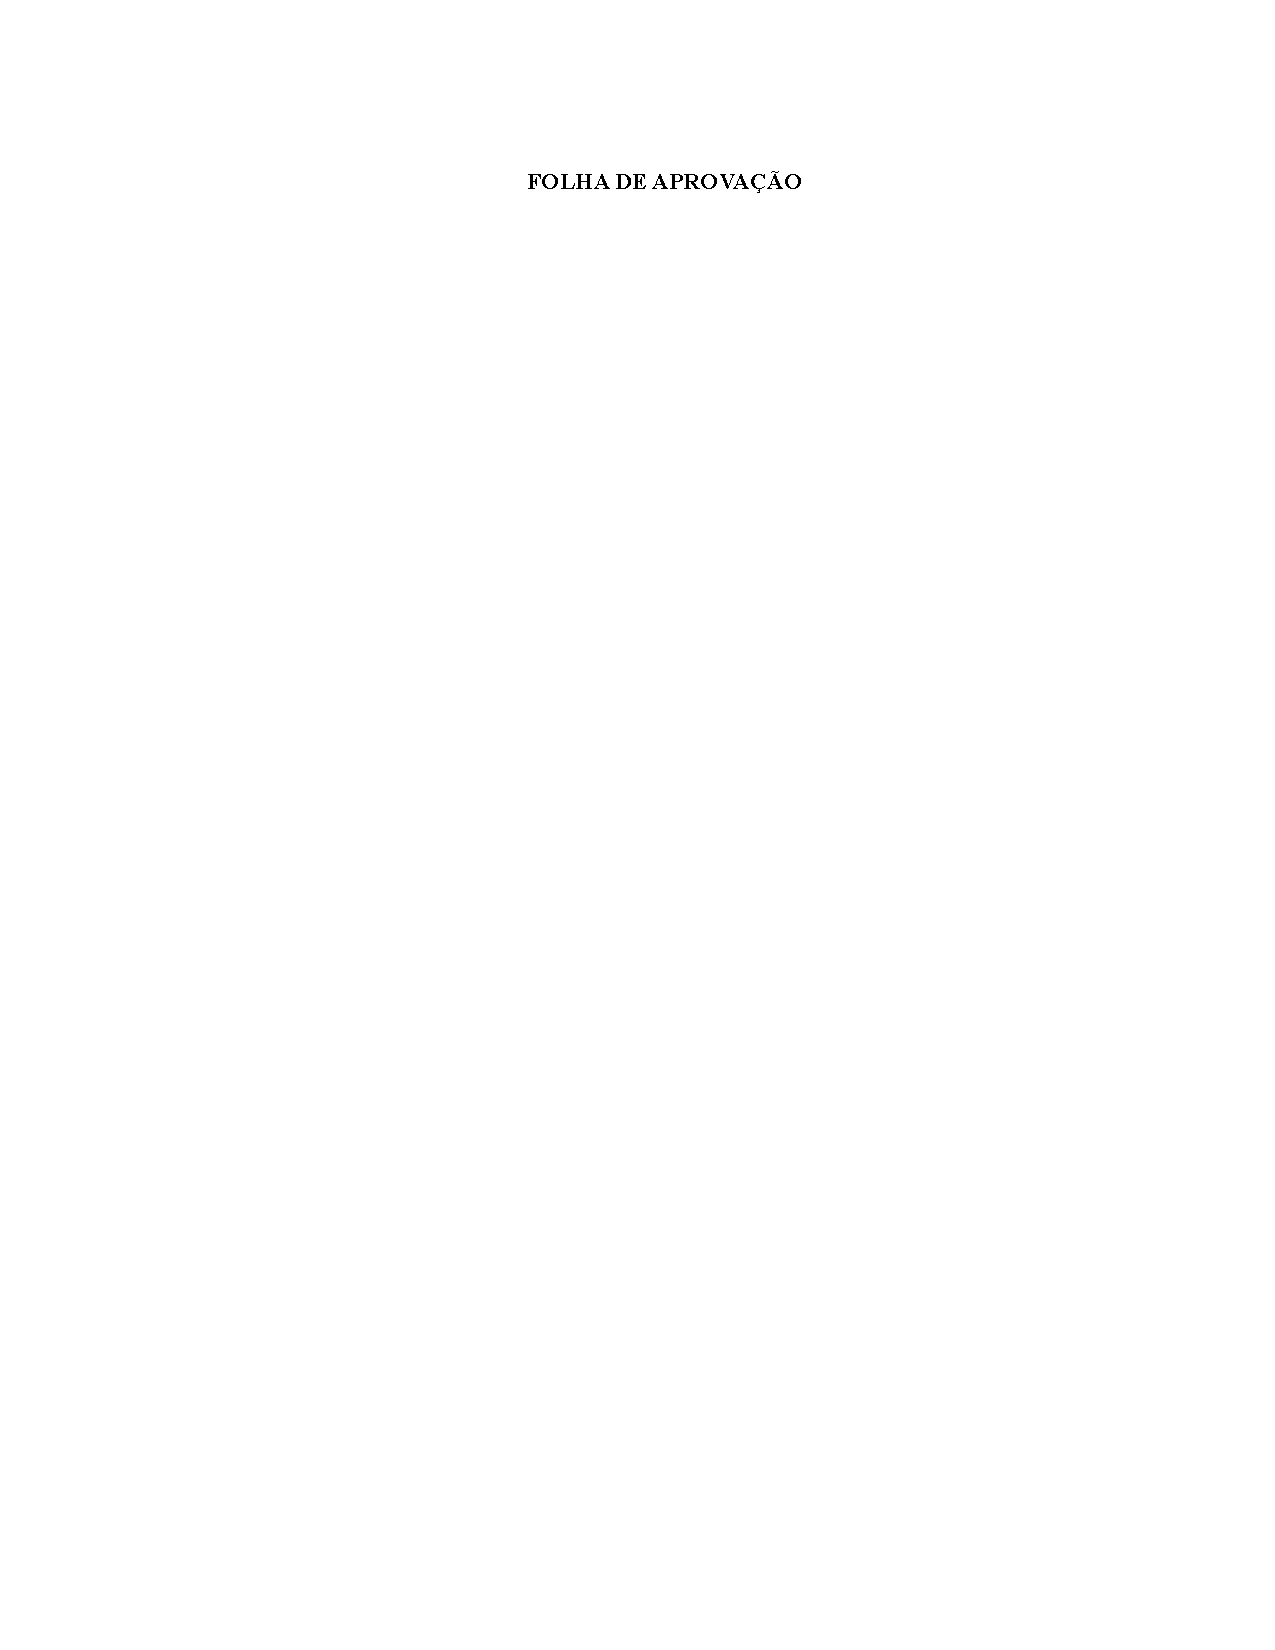
\includepdf[scale=1.0,pages=1]{./PreTexto/folha-aprovacao.pdf} % para adicionar o pdf enviado pelo professor apenas substitua o documento folha-aprovacao.pdf dentro da pasta PreTexto

%% Dedicatória
%%%% DEDICATÓRIA
%%
%% Texto em que o autor presta homenagem ou dedica seu trabalho.

\begin{dedicatoria}%% Ambiente dedicatoria

\textcolor{red}{Espaço destinado à dedicatória (\underline{elemento opcional}). 
Folha que contém o oferecimento do trabalho à determinada pessoa ou pessoas. \underline{Exemplo:}}
\vspace{1cm}

Dedico este trabalho à minha família, pelos momentos de ausência.

\end{dedicatoria}
%% Comente para remover este item

%% Agradecimentos
%%%% AGRADECIMENTOS
%%
%% Texto em que o autor faz agradecimentos dirigidos àqueles que contribuíram de maneira relevante à elaboração do trabalho.

\begin{agradecimentos}%% Ambiente agradecimentos

Certamente estes parágrafos não irão atender a todas as pessoas que fizeram parte dessa importante fase de minha vida. Portanto, desde já peço desculpas àquelas que não estão presentes entre essas palavras, mas elas podem estar certas que fazem parte do meu pensamento e de minha gratidão. 

Agradeço ao(a) meu(minha) orientador(a) Prof.(a) Dr.(a) Nome Completo, pela sabedoria com que me guiou nesta trajetória.

Aos meus colegas de sala.

A Secretaria do Curso, pela cooperação.

Gostaria de deixar registrado também, o meu reconhecimento à minha família, pois acredito que sem o apoio deles seria muito difícil vencer esse desafio. 

O presente trabalho foi realizado com apoio da Coordenação de Aperfeiçoamento de Pessoal de Nível Superior - Brasil (CAPES) - Código de Financiamento 001

\textcolor{red}{Equivalente para trabalhos escritos em língua inglesa:} This study was financed in part by the Coordenação de Aperfeiçoamento de Pessoal de Nível Superior - Brasil (CAPES) - Finance Code 001.

Enfim, a todos os que por algum motivo contribuíram para a realização desta pesquisa.

\singlespacing{
\vspace{0.5cm}
\noindent\small\textcolor{red}{Espaço destinado aos agradecimentos (\underline{elemento opcional}). Folha que contém manifestação de reconhecimento a pessoas e/ou instituições que realmente contribuíram com o(a) autor(a), devendo ser expressos de maneira simples.}

\vspace{0.3cm}
\noindent\small\textcolor{red}{Não devem ser incluídas informações que nominem empresas ou instituições não nominadas no trabalho.}

\vspace{0.3cm}
\noindent\small\textcolor{red}{\textbf{Os trabalhos que receberam fomento da UTFPR ou de qualquer agência de fomento, a exemplo de CAPES, CNPq e Fundação Araucária, deverão conter, no último parágrafo dos Agradecimentos, o nome da agência, bem como o número do financiamento}. Este item deve ser o último.}

\vspace{0.3cm}
\noindent\small\textcolor{red}{Atenção: não utilizar este exemplo na versão final. Use a sua criatividade faça os seus próprios agradecimentos!}
}


\end{agradecimentos}
%% Comente para remover este item

%% Epígrafe
%%%% EPÍGRAFE
%%
%% Texto em que o autor apresenta uma citação, seguida de indicação de autoria, relacionada com a matéria tratada no corpo do
%% trabalho.
\begin{epigrafe}%% Ambiente epigrafe


\hspace{-10cm}\parbox{16cm}{\textcolor{red}{\small \singlespacing{Espaço destinado à epígrafe (\underline{elemento opcional}). Neste espaço, o(a) autor(a) usa uma citação, seguida de indicação de autoria e ano, relacionada, preferencialmente, com o assunto tratado no corpo do trabalho. \textbf{Esta citação deverá constar na lista de referências}. \underline{Exemplo:} \vspace{0.5cm}}}
}

``A biblioteca é um jardim onde as ideias florescem e os frutos são colhidos pela eternidade.'' \cite{Candido2002}.
\end{epigrafe}
%% Comente para remover este item

%% Resumo
%%%% RESUMO
%%
%% Apresentação concisa dos pontos relevantes de um texto, fornecendo uma visão rápida e clara do conteúdo e das conclusões do
%% trabalho.

\begin{resumoutfpr}%% Ambiente resumoutfpr
O resumo deve ressaltar de forma sucinta o conteúdo do trabalho, incluindo justificativa, objetivos, metodologia, resultados e conclusão. Deve ser redigido em um único parágrafo, justificado, contendo de 150 \textbf{até 500 palavras. Evitar incluir citações, fórmulas, equações e símbolos} no resumo.As palavras-chave e as keywords são grafadas em inicial minúscula quando não forem nome próprio ou nome científico e separados por ponto e vírgula.

\singlespacing{\textcolor{red}{\footnotesize De acordo com a NBR 6028:2021, a apresentação gráfica deve seguir o padrão do documento no qual o resumo está inserido. Para definição das palavras-chave (e suas correspondentes em inglês no abstract) consultar em Termo tópico do \textbf{Catálogo de Autoridades} da Biblioteca Nacional, disponível em:} \footnotesize{http://acervo.bn.gov.br/sophia\_web/autoridade.}}
\end{resumoutfpr}

%% Comente para remover este item

%% Abstract
%%%% ABSTRACT
%%
%% Versão do resumo para idioma de divulgação internacional.

\begin{abstractutfpr}%% Ambiente abstractutfpr
Seguir o mesmo padrão do resumo, com a tradução do texto do resumo e referência, se houver, para a língua estrangeira (língua inglesa).
\end{abstractutfpr}
%% Comente para remover este item

%% Lista de algoritmos
%\incluirlistadealgoritmos%% Comente para remover este item


%% Lista de Ilustrações
%% Figuras, Gráficos, Quadros e Fotografias são incluídos juntos em uma mesma lista
%% Na UTFPR sugere-se adotar listas próprias, conforme a natureza da ilustração, a partir da existência de 3 elementos da mesma natureza.Neste caso, cada lista deverá iniciar em folha distinta. Não criar listas com apenas um item.


\incluirlistadeilustracoes


%% Lista de figuras
%\incluirlistadefiguras%% Comente para remover este item

%\incluirlistageraldeilustracoes
%\listofgeneralilust



%% Lista de Fotografias
%\incluirlistadefotografias %% Comente para remover este item


%% Lista de Gráficos
%\incluirlistadegraficos %% Comente para remover este item

%% Lista de tabelas
\incluirlistadetabelas%% Comente para remover este item

%% Lista de quadros
%\incluirlistadequadros

%% Listagem de códigos fonte
%\incluirlistadecodigosfonte

%% Lista de abreviaturas, siglas e acrônimos
\incluirlistadeacronimos{file}%% Opções: "glossaries" (pacote) ou "file" (arquivo) ou "none" (desabilita)

%% Lista de símbolos
\incluirlistadesimbolos{file}%% Opções: "nomencl" (pacote) ou "file" (arquivo) ou "none" (desabilita)

%% Sumário
\incluirsumario%% Comente para remover este item

%% Formatação de páginas de elementos textuais
\textual%% Não comente esta linha

%% Parte
% \part{Introdução}%% Comente para remover este item

%% Capítulo introdução - obrigatório
%%%% CAPÍTULO 1 - INTRODUÇÃO
%%
%% Deve apresentar uma visão global da pesquisa, incluindo: breve histórico, importância e justificativa da escolha do tema,
%% delimitações do assunto, formulação de hipóteses e objetivos da pesquisa e estrutura do trabalho.

%% Título e rótulo de capítulo (rótulos não devem conter caracteres especiais, acentuados ou cedilha)
\chapter{Introdução}\label{cap:introducao}

Parte inicial do texto, na qual devem constar o tema e a delimitação do assunto tratado, objetivos da pesquisa e outros elementos necessários para situar o tema do trabalho. \textcolor{red}{Após o início de uma seção, recomenda-se a inserção de um texto ou, no mínimo, uma nota explicativa sobre a seção iniciada. Evitar, por exemplo:}

% Segundo \citeonline{Coulouris2013}.

% Segundo \citeonline[p. 40]{Coulouris2013}.

% Citação no final do Parágrafo~\cite{Coulouris2013}. 

% Citação no final do Parágrafo com número de página~\cite[p. 40]{Coulouris2013}.

% %(Modelo de referência: pessoa jurídica)
% Citação no final do Parágrafo~\cite{NBR6023:2018}

% %(Modelo de referência: pessoa jurídica)
% Citação no final do Parágrafo~\cite{NBR6027:2012}

% %(Modelo de referência: pessoa jurídica)
% Citação no final do Parágrafo~\cite{NBR6028:2021}

% Segundo a \citeonline{NBR14724:2011}.

% Citação no final do Parágrafo~\cite{NBR10520:2002}

% Citação no final do Parágrafo~\cite{NBR14724:2011}.

% % (Modelo de referência de trabalho acadêmico).
% Citação no final do Parágrafo~\cite{Andrade2005}

% % (Modelo de referência: capítulo de livro).
% Citação no final do Parágrafo~\cite{Borges2014}

% % (Modelo de referência: leis, decretos, portarias, etc.)
% Citação no final do Parágrafo~\cite{BRASIL:1998}

% % (Modelo de referência: livro com subtítulo). Nome com sufixo "Von" - Configuração no bib
% Citação no final do Parágrafo~\cite[p. 66]{KROGH:2001}

% Citação no final do Parágrafo~\cite{Faina2001}

% % (Modelo de referência: livro com subtítulo).
% Citação no final do Parágrafo~\cite{Davenport2012}

% % (Modelo de referência: artigo de periódico).
% Citação no final do Parágrafo~\cite{Monteiro2009}

% %(Modelo de referência: artigo de periódico). Nome familiar "Junior"
% Citação no final do Parágrafo~\cite{Sanches2024}

% % (Modelo de referência: trabalho publicado em evento).
% Citação no final do Parágrafo~\cite{Renaux2001}

\section{Contextualização}

\subsection{Memorial de Pesquisa}


\section{Paginação}

Todas as folhas do trabalho, a partir da folha de rosto, devem ser contadas sequencialmente, mas não numeradas. A numeração deve ser inserida à partir da primeira folha da parte textual (Introdução), em algarismos arábicos, no canto superior direito da folha. Havendo apêndices e anexos, as suas folhas devem ser paginadas de maneira contínua.

\section{Exemplos de utilização de numeração progressiva}

Nos títulos com indicativo numérico não se utilizam pontos, hífen, travessão, ou qualquer sinal após o indicativo de seção ou de título. 

A numeração progressiva para as seções do texto deve ser adotada para evidenciar a sistematização do conteúdo do trabalho. 

Destacam-se gradativamente os títulos das seções, utilizando-se tipograficamente com recursos como letra maiúscula, negrito, itálico ou sublinhado. 

No sumário, os títulos devem aparecer de forma idêntica ao texto.

\textcolor{red}{Ver os exemplos na folha seguinte:}

%% Comente para remover este item


%%
\chapter{Seção primária (CAIXA ALTA e NEGRITO)}

As seções primárias devem iniciar sempreem páginas distintas. Entre uma seção e outra sempre haverá um texto.

\textcolor{red}{Texto justificado, com recuo especial na primeira linha de 1,5 cm. Não utilizar tab (1,25 cm). Os títulos das seções devem ser separados do texto que os precede por 1 (um) espaço (1,5 cm).}



\section{Seção secundária (negrito)}
Texto, texto, texto, texto, texto, texto, texto, texto, texto, texto, texto, texto, texto, texto, texto, texto, texto, texto, texto, texto, texto, texto, texto, texto, texto.


\subsection{Seção terciária (sem negrito)}

Texto, texto, texto, texto, texto, texto, texto, texto, texto, texto, texto, texto, texto, texto, texto, texto, texto, texto, texto, texto, texto, texto, texto, texto, texto.



 
\subsubsection{Seção quaternária (sublinhado)}
Texto, texto, texto, texto, texto, texto, texto, texto, texto, texto, texto, texto, texto, texto, texto, texto, texto, texto, texto, texto, texto, texto, texto, texto, texto.


\subsubsubsection{Seção quinária (itálico)}
Texto, texto, texto, texto, texto, texto, texto, texto, texto, texto, texto, texto, texto, texto, texto, texto, texto, texto, texto, texto, texto, texto, texto, texto, texto.



% ******************************

% Em relação ao assunto, o apresentado nesta seção pode estar relacionado a trabalhos de outros autores ou ao assunto que fornece a fundamentação (motivação) para o trabalho a ser desenvolvido. Se o assunto está relacionado a trabalhos de outros autores, a contribuição do trabalho é definida em relação ao que já foi pesquisado nesse assunto. Se o assunto será utilizado para embasamento do que será proposto, explicitar como o trabalho se insere nesse assunto. A contribuição pode, ainda, estar relacionada a uma necessidade de mercado ou a uma oportunidade decorrente de algum problema real para o qual se pretender propor uma solução. Nesse caso, o assunto fornece um contexto teórico de suporte para o problema e/ou a solução.

% O importante nesta seção é deixar claro do que se trata o trabalho (assunto ou tema), identificar o objeto de pesquisa, como será encaminhada a solução (procedimento metodológico, tecnologias, ferramentas utilizadas) e o que se pretende ao final do trabalho, sem explicitar a solução e os resultados.

% \caixa{Atenção}{As seções a seguir são sugestões, converse com o seu orientador para ver quais seções devem ter em seu trabalho!}

% \begin{photograph}[!htb]%% Ambiente figure
%     %\captionsetup{width=0.55\textwidth}%% Largura da legenda
%     \caption{Exemplo de fotografia}%% Legenda
%     \label{fig:exemplo1}%% Rótulo
%     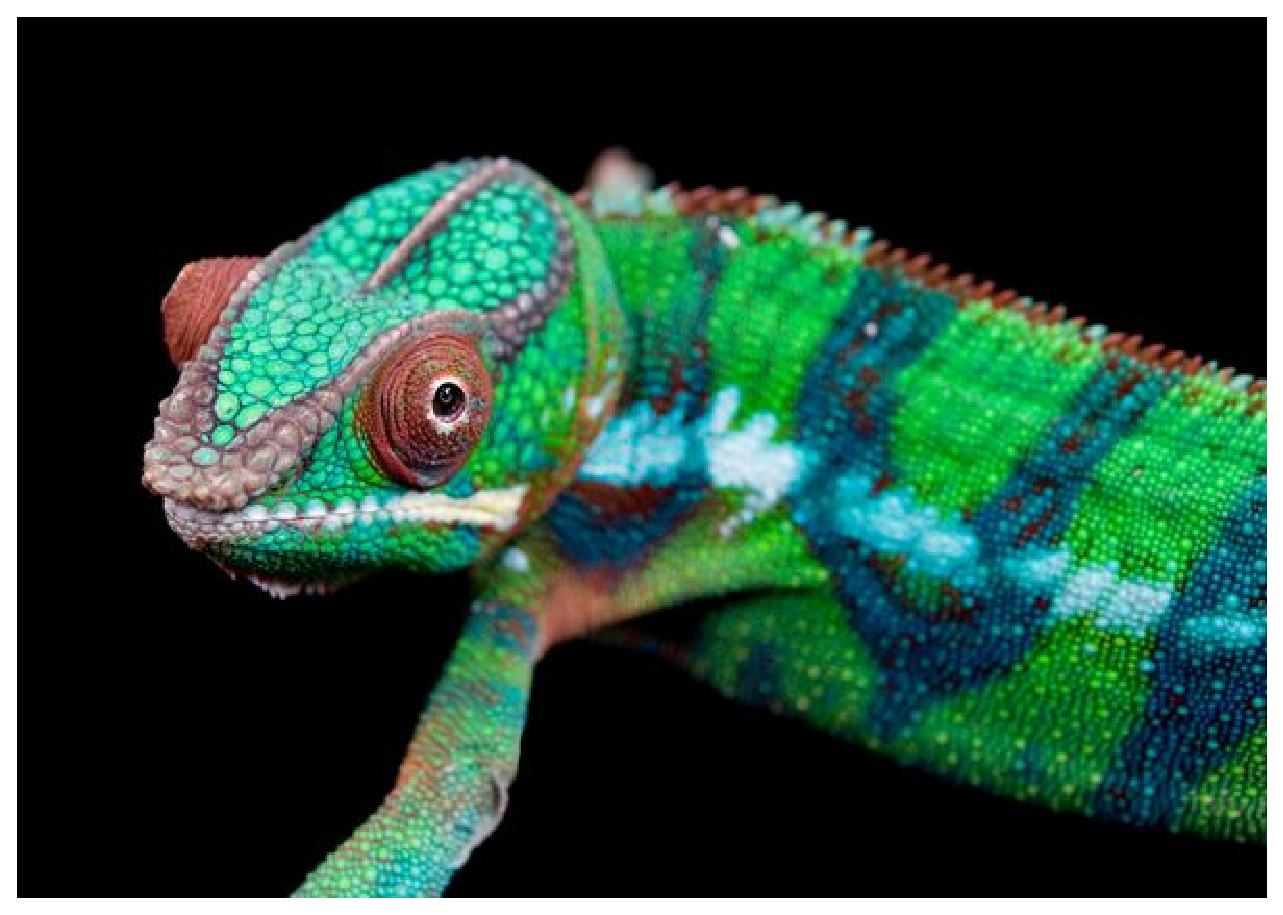
\includegraphics[scale=0.4]{foto1}%% Dimensões e localização
%     \fonte{Autoria Própria}%% Fonte
%     \addcontentsline{loge}{photograph}{\protect\numberline{\thephotograph}Exemplo de fotografia.} % Adiciona à lista de ilustrações
% \end{photograph}


% \section{Objetivos}\label{sec:objetivos}

% Um texto curto\footnote{Teste de nota de rodapé 1.} apresentando a seção.



% \section{Objetivos específicos (opcional)}\label{subsec:objetivosEspecificos}

% Os objetivos específicos são opcionais, ou seja, somente devem ser apresentados se caracterizarem resultados parciais gerados a partir do objetivo geral, os quais sejam considerados úteis para a comunidade acadêmica, para a sociedade ou para o ambiente profissional. Uma observação importante é que os resultados sejam passíveis de comprovação, ou seja, se o objetivo for: “Oferecer agilidade e confiabilidade aos processos gerenciais da empresa”, significa que o trabalho deverá realizar testes com relação a esses atributos, cujos resultados deverão ser apresentados nas discussões do trabalho.

% \begin{graph}[!htb]%% Ambiente figure
%     %\captionsetup{width=0.55\textwidth}%% Largura da legenda
%     \caption{Exemplo de gráfico}%% Legenda
%     \label{graph1}%% Rótulo
%     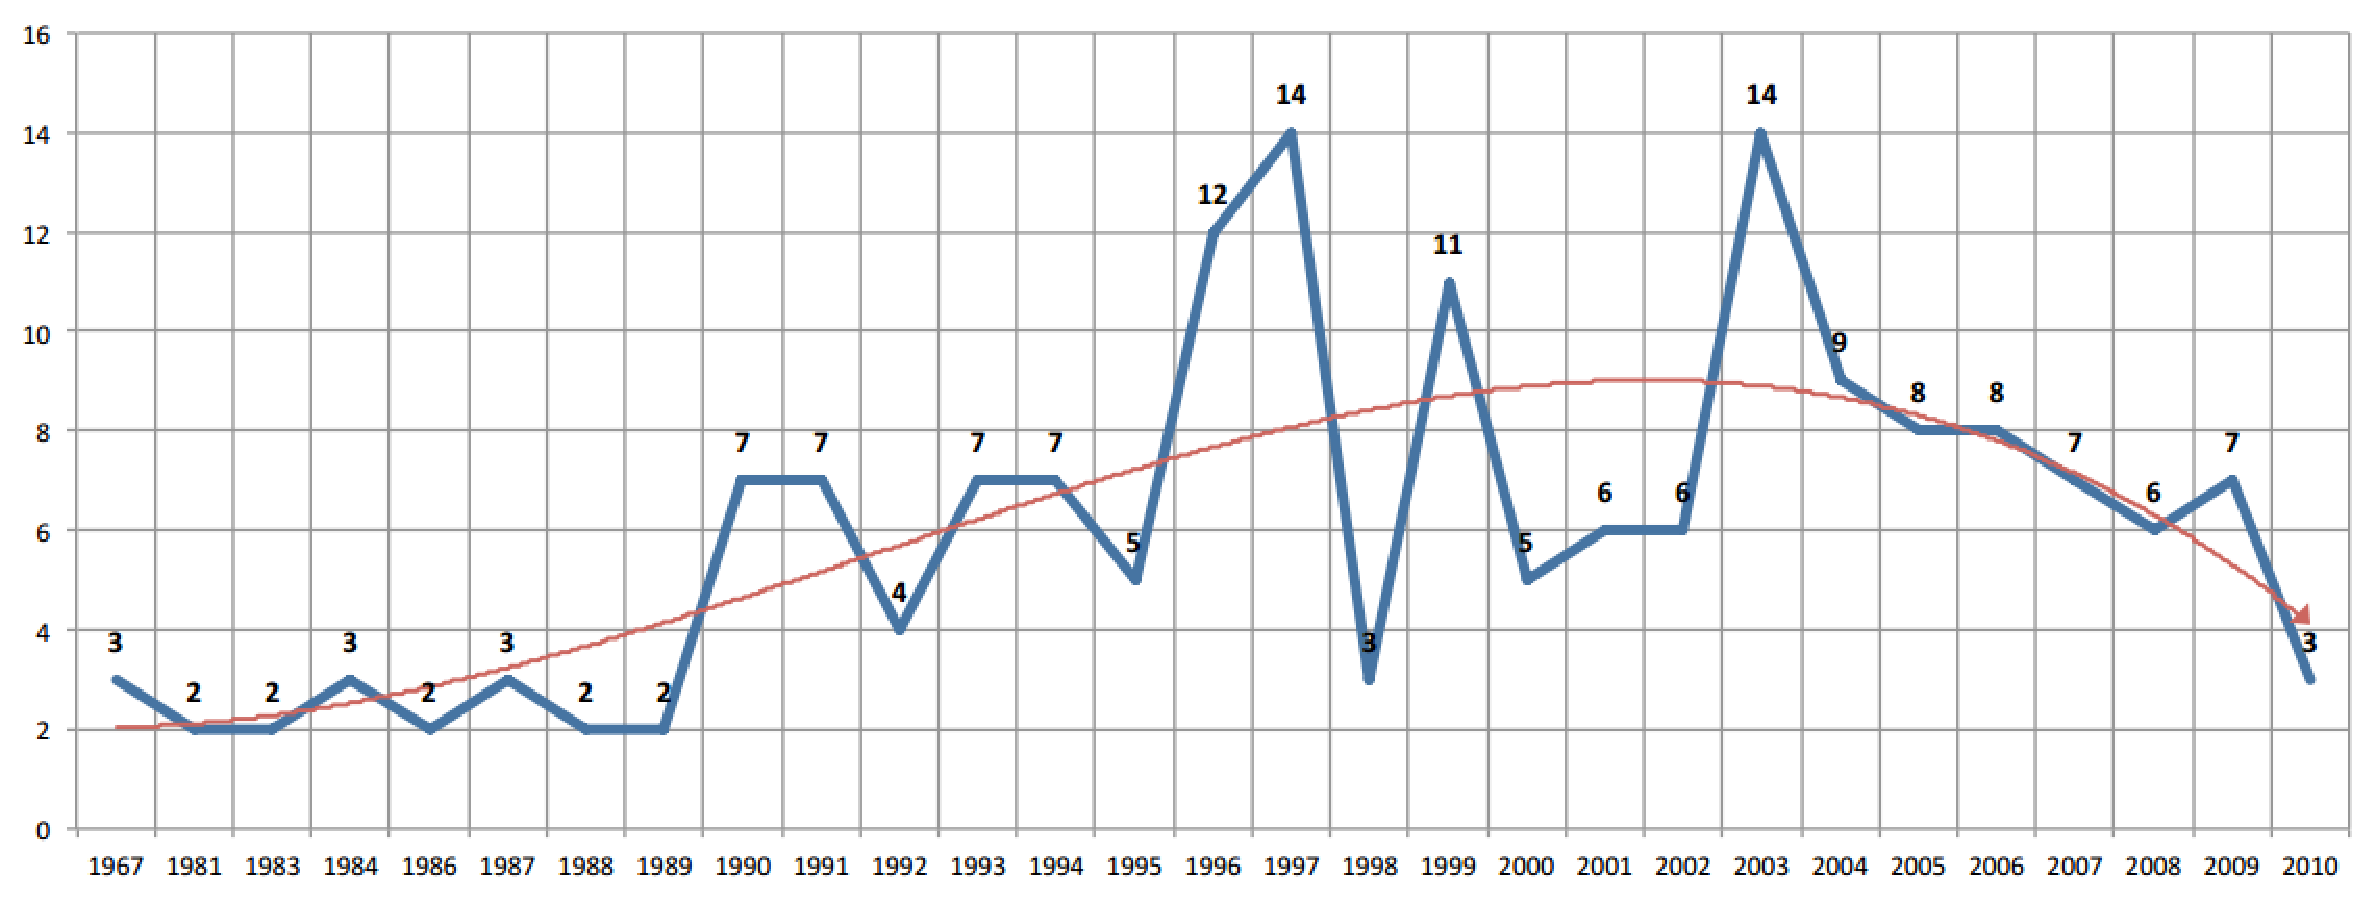
\includegraphics[scale=0.4]{grafico2}%% Dimensões e localização
%     \fonte{Adaptado de \citeonline[p.~4]{UTFPR2008}}%% Fonte
%     \addcontentsline{loge}{graph}{\protect\numberline{\thegraph}Exemplo de gráfico.}
% \end{graph}


% Destaca-se que os objetivos específicos não incluem as etapas do processo de desenvolvimento de software (realizar a modelagem, a análise, o projeto...) ou outras atividades necessárias para alcançar o objetivo geral, como, estudar as tecnologias necessárias para modelagem e implementação do sistema. Dentre as exceções estão a realização de estudos, procedimentos, métodos e técnicas considerados inéditos e de relevância para outros trabalhos a serem realizados na mesma área. Contudo, o resultado deste estudo deve ser documentado de forma que seja conhecimento disponibilizado para quem lê o trabalho.


% \section{Justificativa}\label{sec:justificativa}

% Justificar o objeto de pesquisa (o que será feito) e a forma de resolução do problema (como fazer). A forma de resolução pode estar centrada no método, nas tecnologias, no uso de conceitos (fundamentação teórica).

% A Justificativa explicita porque desenvolver o referido trabalho, como o mesmo se insere no contexto de pesquisa, de produção científica. Pode incluir o porquê utilizar as tecnologias e ferramentas indicadas, a contribuição em termos de inovação ou mesmo de aprendizado.

% O trabalho não precisa ser justificado em decorrência de ser inovador ou por ter gerado uma significativa contribuição ao conhecimento na área em que o mesmo se insere. Pode referir-se simplesmente à aplicabilidade de conhecimentos adquiridos durante o curso. Sendo assim, a justificativa não deve ser elaborada considerando um mercado a ser atingido e sim com relação ao uso de tecnologias aprendidas e/ou estudadas, o conhecimento e aprendizado do aluno e a aplicabilidade do trabalho desenvolvido.

% \section{Estrutura do trabalho}\label{sec:estruturaTrabalho}

% A estrutura do trabalho contém uma relação dos capítulos e uma descrição sucinta do que cada um deles contém. Esta seção fornece uma visão geral do trabalho no sentido da sua estrutura em capítulos\footnote{Teste de nota de rodapé 2.}.

% \caixa{Atenção}{O OverLeaf está demorando muito para compilar o modelo com o Capítulo de Exemplos, que explica como usar o LaTeX. Assim, esse capítulo foi removido (está comentado para não compilar), mas há um arquivo chamado \texttt{exemploPDF.pdf}, na raiz do projeto, que contém esse capítulo de exemplos!}




%% Capítulo
\chapter{Desenvolvimento}

Parte principal do trabalho, que contém a exposição ordenada e pormenorizada do assunto. É composta de revisão de literatura, dividida em seções e subseções, material e métodos e/ou metodologia e resultados, agora descritos detalhadamente. Cada seção ou subseção deverá ter um título apropriado ao conteúdo.

Deve-se utilizar sempre a terceira pessoa do singular na elaboração do texto, mantendo-se a forma impessoal.

\section{Regras gerais de apresentação}

Constituem-se como padrão para apresentação de trabalhos acadêmicos:

\begin{itemize}
\item Tamanho da fonte: Arial ou Times New Roman, tamanho 12. Deve-se utilizar apenas um dos tipos escolhidos em todo o trabalho. Fonte tamanho 10 para citações de mais de três linhas, notas de rodapé e legendas, corpo e fonte das ilustrações e tabelas e paginação.
\item Formato do título: o título do trabalho, na capa e na folha de rosto, deve aparecer em CAIXA ALTA, negrito, centralizado e fonte tamanho 12. Havendo subtítulo, este deve ser precedido por dois pontos, escrito também em CAIXA ALTA, negrito e sem ponto final;
\item Parágrafo: com recuo na primeira linha de 1,5 cm., justificado, sem espaçamento anterior ou posterior.
\end{itemize}

\section{Margens}
Utilizar margens esquerda e superior de 3 cm; e margens direita e inferior de 2 cm; Tamanho do papel: A4; Cabeçalho e rodapé: 1,25 cm.

\section{Espaçamento}

As notas, as referências e a natureza do trabalho devem ser digitadas em espaço simples; Todo o texto deve ser formatado com espaço de 1,5 cm entre linhas (sem espaçamento antes/depois).

As citações com mais de três linhas (longas) são em espaço simples e com recuo de 4 cm da margem esquerda. ``As referências devem ser elaboradas em espaço simples, alinhadas à margem esquerda do texto e separadas entre si por uma linha em branco de espaço simples''~\cite{NBR6023:2018}.

\section{Ilustrações}

São ilustrações: f\textbf{iguras, quadros, gráficos, fotografias}, retratos, desenhos, gravuras, imagens, fluxogramas, organogramas, esquemas, mapas, plantas e \textbf{diferenciam-se das tabelas}. As ilustrações devem ser inseridas o mais próximo possível do texto a que se refere, mas mantendo um espaço (1,5 cm) de separação.

Qualquer que seja o tipo de ilustração, sua identificação deve ser posicionada na parte \textbf{superior}, precedida da palavra designativa, seguida de seu número de ordem de ocorrência no texto, em algarismos arábicos, do respectivo título e/ou legenda. A fonte deve ser tamanho 10. Após a legenda, deve-se apresentar ilustração e em seguida citar a fonte de onde foi retirada a ilustração, exemplo: Fonte: Autor (data), bem comodeve-se referenciá-la, de forma completa, na seção Referências. 

* Para inserir legendas nas ilustrações e tabelas: 

\begin{enumerate}
    \item Na guia \textbf{Referências}, no grupo \textbf{Legendas}, clicar em \textbf{Inserir Legenda}.
    \item Na lista \textbf{Rótulo}, selecionar o rótulo que descreve melhor o objeto. Se a lista não contiver o rótulo correto, clicar em \textbf{Novo Rótulo}, digitar o novo rótulo na caixa \textbf{Rótulo} e clicar em \textbf{OK}.
    \item Digitar o texto, incluindo a pontuação que deseja exibir depois do rótulo e clicar \textbf{enter} para utilizar a formatação apropriada para a Fonte.
\end{enumerate}

\textcolor{red}{Utilizar sempre a primeira linha da folha, em todo o trabalho. A seguir, um modelo de formatação de figura:}

\newpage



\begin{figure}[!htb]%% Ambiente figure
     %\captionsetup{width=0.55\textwidth}%% Largura da legenda
     \caption{As dimensões curriculares de pré-escolar}%% Legenda
     \label{fig:exemplo2}%% Rótulo
     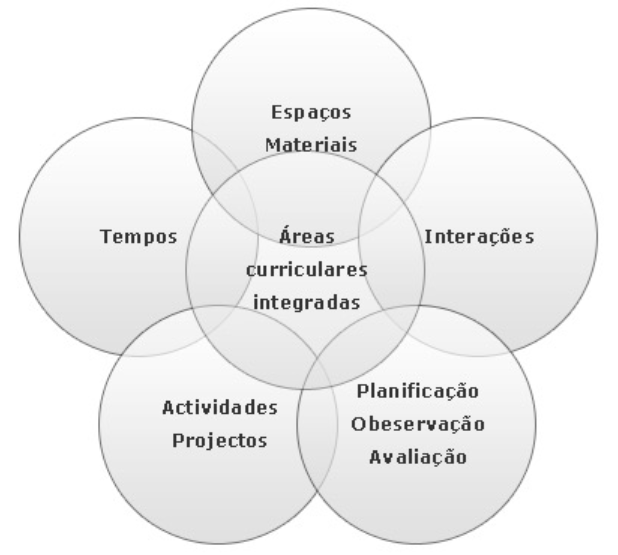
\includegraphics[scale=0.5]{FigDimCurriculares}%% Dimensões e localização
     \fonte{\citeonline{Centro:2025}}%% Fonte
     \addcontentsline{loge}{figure}{\protect\numberline{\thefigure}As dimensões curriculares de pré-escolar}
 \end{figure}

Texto, texto, texto, texto, texto, texto, texto, texto, texto, texto, texto, texto.


\begin{figure}[!htb]%% Ambiente figure
     %\captionsetup{width=0.55\textwidth}%% Largura da legenda
     \caption{Glândulas exócrinas e endócrinas}%% Legenda
     \label{fig:exemplo3}%% Rótulo
     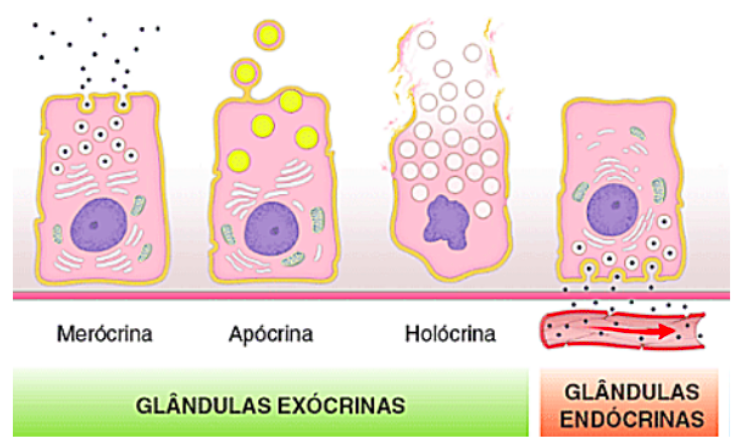
\includegraphics[scale=0.5]{glandulas}%% Dimensões e localização
     \fonte{Adaptado de \citeonline[p.~144]{Pawlina:2018}}%% Fonte
     \addcontentsline{loge}{figure}{\protect\numberline{\thefigure}Glândulas exócrinas e endócrinas}
 \end{figure}


\noindent\textcolor{red}{A seguir, um modelo de formatação de fotografia:}

\newpage

 \begin{photograph}[!htb]%% Ambiente figure
      %\captionsetup{width=0.55\textwidth}%% Largura da legenda
      \caption{Entrada do antigo Departamento de Biblioteca da UTFPR Campus Ponta Grossa}%% Legenda
      \label{fig:foto1}%% Rótulo
      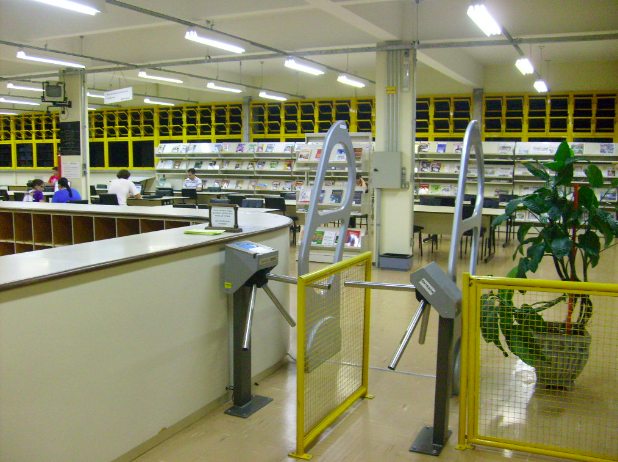
\includegraphics[scale=0.5]{fotografia1}%% Dimensões e localização
      \fonte{Autoria própria (2014)}%% Fonte
      \addcontentsline{loge}{photograph}{\protect\numberline{\thephotograph}Entrada do antigo Departamento de Biblioteca da UTFPR Campus Ponta Grossa} % Adiciona à lista de ilustrações
  \end{photograph}

\noindent\textcolor{red}{\textbf{Atenção:} As fontes das ilustrações e tabelas também deverão constar na lista de referências, ou indicar como Fonte: Autoria própria (ano), se for o caso. Na UTFPR adotou-se negrito e centralizado nas legendas e fonte das ilustrações e tabelas.}

 \begin{photograph}[!htb]%% Ambiente figure
      %\captionsetup{width=0.55\textwidth}%% Largura da legenda
      \centering
      \caption{Entrada da Biblioteca Mario Vargas Llosa, Lima (Peru), também conhecida como ``Casa de la Literatura Peruana''. Em destaque, o primeiro tipógrafo adquirido na América Latina}%% Legenda
      \label{fig:foto2}%% Rótulo
      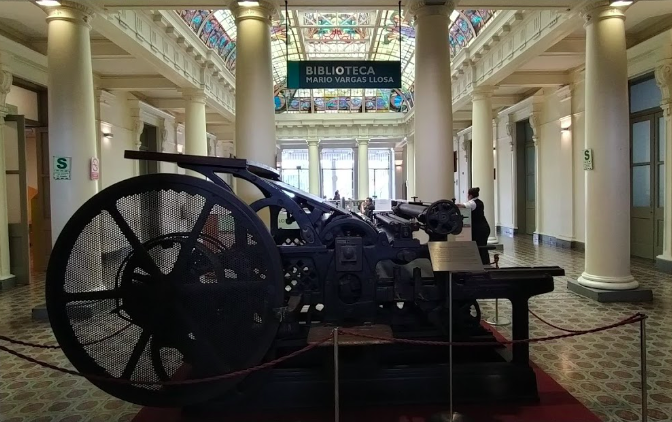
\includegraphics[scale=0.5]{fotografia2}%% Dimensões e localização
      \fonte{Autoria própria (2019)}%% Fonte
      \addcontentsline{loge}{photograph}{\protect\numberline{\thephotograph}Entrada da Biblioteca Mario Vargas Llosa, Lima (Peru), também conhecida como ``Casa de la Literatura Peruana''. Em destaque, o primeiro tipógrafo adquirido na América Latina} % Adiciona à lista de ilustrações
  \end{photograph}

 \textcolor{red}{A seguir, um modelo de formatação de gráfico:}

 \newpage

 \begin{graph}[!htb]%% Ambiente figure
      %\captionsetup{width=0.55\textwidth}%% Largura da legenda
      \caption{Estatística de empréstimos domiciliares realizados em janeiro de 2019 pelas Bibliotecas da UTFPR}%% Legenda
      \label{fig:grap1}%% Rótulo
      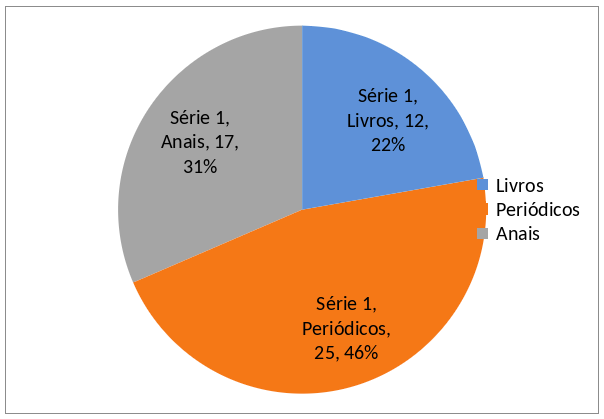
\includegraphics[scale=0.5]{grafico1a}%% Dimensões e localização
      \fonte{\citeonline{UTFPR2020}}%% Fonte
      \addcontentsline{loge}{graph}{\protect\numberline{\thephotograph}Estatística de empréstimos domiciliares realizados em janeiro de 2019 pelas Bibliotecas da UTFPR} % Adiciona à lista de ilustrações
  \end{graph}

Texto, texto, texto, texto, texto, texto, texto, texto, texto, texto, texto, texto, texto, texto, texto, texto, texto, texto, texto, texto, texto, texto, texto, texto, texto.

\textcolor{red}{Modelo de formatação de quadros (prevalecem informações textuais).}

\begin{tabframed}[htb]%% Ambiente tabframed
 %\captionsetup{width=0.5\textwidth}%% Largura da legenda
 \caption{Áreas de desenvolvimento de competências na organizações (pública e privada)}%% Legenda
 \label{quad:exemplo1}%% Rótulo
 \renewcommand{\arraystretch}{1.5}
 \begin{tabular}{|l|p{9cm}|}
 \cline{1-2}
 \multicolumn{1}{|c|}{\textbf{Áreas de desenvolvimento}} & \multicolumn{1}{|c|}{\textbf{\centering Descrição}}\\ \cline{1-2}
  1. Competências sobre processos & Conhecimento nos processos de trabalho \\ \cline{1-2}  
  2. Competências técnicas & Conhecimento técnico nas tarefas a serem desempenhadas e tecnologias empregadas nestas tarefas \\ \cline{1-2}  
  3. Competências sobre a organização & Saber organizar os fluxos de trabalho \\ \cline{1-2}
  4. Competências de serviço & Aliar as competências técnicas com o impacto que estas ações terão para o cliente consumidor \\ \cline{1-2}
  5. Competências sociais & Atitudes que sustentam o comportamento do indivíduo: saber comunicar-se e responsabilizar-se pelos seus atos.\\ \cline{1-2}
 \end{tabular}
 \fonte{\citeonline{FLEURY:2018}}%% Fonte
 \addcontentsline{loge}{tabframed}{\protect\numberline{\thetabframed}Áreas de desenvolvimento de competências na organizações (pública e privada)}
 \end{tabframed}

\textcolor{red}{Para quadros que ocupam mais de uma folha, não é necessária nenhuma sinalização (continua/continuação/conclusão). Apenas nas tabelas se faz necessária essa sinalização}

Texto, texto, texto, texto, texto, texto, texto, texto, texto, texto, texto, texto.

\newpage

\section{Tabelas}

Deve-se seguir tal padrão em todo o trabalho, constando também na lista de tabelas, separada da lista de ilustrações. \textcolor{red}{As tabelas se diferenciam dos quadros por não apresentarem os fechamentos laterais.}\footnote{Para as regras gerais de apresentação das tabelas consultar: IBGE (Instituto Brasileiro de Geografia e Estatística). \textbf{Normas para Apresentação Tabular}. 3. ed. Rio de Janeiro: IBGE, 1993. Disponível em: http://biblioteca.ibge.gov.br/visualizacao/livros/liv23907.pdf
}

\vspace{1cm}

\textcolor{red}{Modelo de formatação de tabelas (prevalecem informações numéricas).}


\begin{table}[!htb]
 % Luiz - O texto do caption da tabela/quadro deve ser do tamanho da tabela, então utilize a linha a seguir para conseguir esse efeito
 \captionsetup{width=0.83\textwidth}
 \centering
 \caption{\label{tab:exemplo1}Desempenho dos alunos na prova de conhecimentos específicos, por área do conhecimento}
 \begin{tabular}{p{6cm} cccc}
 	\hline
 	    \multicolumn{1}{c}{\textbf{Média}} & \multicolumn{2}{c}{\textbf{CEFET}} & \multicolumn{2}{c}{\textbf{Peso}} \\ \hline
            \multicolumn{1}{c}{Curso}     & concluintes & ingressantes & concluintes & ingressantes   \\ \hline
            Matemática	    & 27,8	      & 22,5	     & 27,1	        & 22,4 \\
            Letras	        & 32,3	      & 31,5	     & 30,9	         & 26,5 \\
            Geografia	    & 38,4	      & 34,2	     &34,6           &	29,5 \\
            Ciências Biológicas&	26,4  &23,6	         & 26,6	         & 21,9\\ \hline
 \end{tabular}
 \fonte{\citeonline{INEP:2016}}
 \end{table}

Texto, texto, texto, texto, texto, texto, texto, texto, texto, texto, texto, texto, texto, texto, texto, texto, texto, texto, texto, texto, texto, texto, texto, texto, texto. 

Texto, texto, texto, texto, texto, texto, texto, texto, texto, texto, texto, texto, texto, texto, texto, texto, texto, texto, texto, texto, texto, texto, texto, texto, texto. 

Texto, texto, texto, texto, texto, texto, texto, texto, texto, texto, texto, texto, texto, texto, texto, texto, texto, texto, texto, texto, texto, texto, texto, texto, texto.

\vspace{1.5cm}

\textcolor{red}{Para tabelas que ocupam mais de uma folha: deve-se repetir a legenda, na primeira parte não apresentar a linha de fechamento e inserir as sinalizações: continua, continuação (quando ocupar mais de 2 folhas) e conclusão.}

\begin{longtable}{@{\extracolsep{\fill}}p{3cm} c c c}%% Ambiente longtable
 \caption{Situação da educação brasileira em 2002 - Ensino Médio\label{tab:exemplo3}} \\%% Legenda e rótulo
 \multicolumn{4}{r}{\textbf{(continua)}} \\
 \toprule
   &
 \multicolumn{1}{p{3cm}}{\centering \textbf{Taxa de repetência no Ensino Médio (\%)}}&
 \multicolumn{1}{p{3cm}}{\centering \textbf{Taxa de evasão no Ensino Médio (\%)}} & 
 \multicolumn{1}{p{3.5cm}}{\centering \textbf{Taxa de analfabetismo da população de 15 a 17}} \\
 \midrule
 \endfirsthead%% Encerra cabeçalho da primeira página
 \caption*{Situação da educação brasileira em 2002 - Ensino Médio} \\%% Legenda
 \multicolumn{4}{r}{\textbf{(continuação)}} \\
  \toprule
   &
 \multicolumn{1}{p{3cm}}{\centering \textbf{Taxa de repetência no Ensino Médio (\%)}}&
 \multicolumn{1}{p{3cm}}{\centering \textbf{Taxa de evasão no Ensino Médio (\%)}} & 
 \multicolumn{1}{p{3.5cm}}{\centering \textbf{Taxa de analfabetismo da população de 15 a 17}} \\
 \midrule
 \endhead%% Encerra cabeçalho das demais páginas
 %\midrule
 %\multicolumn{4}{r}{\textbf{(continua)}} \\
 \endfoot%% Encerra rodapé das demais páginas
 \bottomrule
 \\[-0.5\linha]
 \caption*{\nomefonte: \citeonline{BRASIL:2014}} \\
 \multicolumn{4}{c}{\textbf{Nota: As notas (quando houver) deverão ser apresentadas após a apresentação da fonte.}}
 \endlastfoot%% Encerra rodapé da última página
  \multicolumn{1}{p{3cm}}{\centering \textbf{Sul}} & ... & ...& ...\\
  \midrule
 Paraná	& 19,3	& 8 &	1,4 \\
 Rio Grande do Sul &	23,3 & 7,7	& 1,1 \\
 Santa Catarina	& 20,6 & 9,5 &	1,4 \\
 \midrule
 \multicolumn{1}{p{3cm}}{\centering \textbf{Sudeste}} & ... & ...& ...\\
 \midrule
 Espírito Santo &	17,4&	5,2&	2,2 \\
 Minas Gerais&	14,2&	7,2&	2,1\\
 Rio de Janeiro&	22,4	&6,5	&1,3\\
 São Paulo	&11,5	&7,6	&0,8\\
 \end{longtable}

\section{Citações}

As regras gerais para apresentação de citações em documentos devem ser consultadas na ABNT NBR 10520:2023 - Informação e documentação - Citações em documentos - Apresentação.

Nesta etapa, é fundamental manter a ética e a honestidade intelectual, garantindo a devida atribuição de autoria a quem realmente contribuiu para o desenvolvimento do estudo. Para isso usa-se as citações, definidas como “menção de uma informação extraída de outra fonte” \cite[p. 1]{NBR10520:2023}.

A transcrição de trechos, seja literal ou parafraseada, torna-se uma citação válida quando acompanhada da devida referência, conforme as normas da ABNT. No entanto, a reprodução de conteúdo sem a atribuição caracteriza-se como plágio, uma prática passível de sanções legais e penais. No Brasil, a Lei n.º 9.610, de 19 de fevereiro de 1998, regula os direitos autorais e estabelece as obrigações aplicáveis. Além disso, o Código Penal, em seu artigo 184, prevê punições para a violação desses direitos.

\subsection{Tipos de citações}

As citações podem ser diretas: transcrição das mesmas palavras utilizadas pelo autor consultado; indiretas: texto baseado na obra do autor consultado e; citação de citação: transcrição de citação direta ou indireta de um texto sem ter acesso a fonte original~\cite[p. 1-2]{NBR10520:2023}.

As citações diretas com até três linhas devem ser inseridas no texto, destacadas entre aspas duplas, precedidas ou sucedidas da indicação de autoria


\newpage
\vspace{0.5cm}\noindent\textbf{Exemplo:}

O autor lembra, contudo, a análise precursora de \citeonline[p. 48]{Barton:1998} sobre alguns “aspectos limitantes das competências, ou aptidões, essenciais, que as transformam em limitações estratégicas”.

As citações diretas com mais de três linhas devem ser destacadas com recuo padronizado de 4 cm em relação a margem esquerda, letra tamanho 10, espaço entrelinhas simples e sem aspas.

\vspace{0.5cm}\noindent\textbf{Exemplo:}

O contexto capacitante não significa necessariamente um espaço físico. Em vez disso, combina aspectos de espaço físico (como o projeto de um escritório ou operações de negócios dispersas), espaço virtual (e-mail, Intranets, teleconferências) e espaço mental (experiências, idéias e emoções compartilhadas). Acima de tudo, trata-se de uma rede de interações, determinada pela solicitude e pela confiança dos participantes \cite[p. 66]{KROGH:2001}.

As citações indiretas não são destacadas mas é preciso indicar a fonte consultada. 

\vspace{0.5cm}\noindent\textbf{Exemplo:}

Vários estudos sobre comportamento informacional dos usuários de bibliotecas universitárias foram identificados (Gonçalves, 2019).

A norma ABNT NBR 10520:2023 estabelece que a expressão apud (palavra em latim que significa: citado por), deve ser utilizada para indicar uma citação de citação, ou seja, quando se cita uma fonte que foi mencionada em outra obra. 

\vspace{0.5cm}\noindent\textbf{Exemplo:}

No modelo serial de Gough (1972 apud Nardi, 1993), o ato de ler envolve um processamento serial que começa com a fixação ocular sobre o texto, prosseguindo da esquerda para a direita de forma linear.

Recomenda-se evitar o uso de apud, pois, com os recursos informacionais disponíveis atualmente, a maioria das obras pode ser consultada diretamente, seja por meio dos acervos das bibliotecas ou pela aquisição do material necessário para o desenvolvimento do estudo.

\newpage
\subsection{Indicação de responsabilidade}

Recomendamos a utilização do sistema autor-data para indicar a responsabilidade de responsabilidade (autoria).

\textbf{Pessoa física:} Sobrenome do autor, em letras maiúscula e minúsculas. Ex.: Silva (2020) ou (Silva, 2020).

\textbf{Pessoa jurídica:} Nome completo, em letras maiúsculas e minúsculas ou sigla da Instituição, em letras maiúsculas. Ex.: Universidade Tecnológica Federal do Paraná, 2020 ou UTFPR, 2020. Na lista de referências a indicação de responsabilidade deve aparecer da mesma maneira que na citação. 

\vspace{0.5cm}\noindent\textbf{Exemplo 1: Sigla}

\noindent No texto:

“Texto texto texto texto texto texto texto texto texto texto” (ABNT, 2018, p. 1). 

\noindent Na lista de referências:

\noindent ABNT. \textbf{ABNT NBR 6023:} informação e documentação: referências: elaboração. Rio de Janeiro: ABNT, 2018.

\vspace{0.5cm}\noindent\textbf{Exemplo 2: Nome por extenso}

\noindent No texto:

“Texto texto texto texto texto texto texto texto texto texto” (ASSOCIAÇÃO BRASILEIRA DE NORMAS TÉCNICAS, 2018, p. 1).

\noindent Na lista de referências:

\noindent ASSOCIAÇÃO BRASILEIRA DE NORMAS TÉCNICAS. \textbf{ABNT NBR 6023:} informação e documentação: referências: elaboração. Rio de Janeiro: ABNT, 2018.

\vspace{0.5cm}\noindent\textbf{Instituição governamental da administração direta: indicar pelo nome do órgão superior ou pelo nome da jurisdição a que pertence}

\vspace{0.5cm}\noindent\textbf{Exemplo:}

\noindent No texto:

“Texto texto texto texto texto texto texto texto texto texto texto” (Brasil, 1995).

\noindent Na lista de referências:
\noindent BRASIL. Ministério da Administração Federal e da Reforma do Estado. \textbf{Plano diretor da reforma do aparelho do Estado.} Brasília, DF: Ministério da Administração Federal e da Reforma do Estado, 1995.

\vspace{0.5cm}\noindent\textbf{Fontes sem autoria ou responsabilidade: indicar pelo título}

\vspace{0.5cm}\noindent\textbf{Exemplo 1: Título composto apenas por uma palavra}

\noindent No texto:

“Texto texto texto texto texto texto texto texto texto texto” (Inglês, 2012).

\noindent Na lista de referências:

\noindent INGLÊS: guia de conversação. São Paulo, Lonely Planet: Globo Livros, 2012.

\vspace{0.5cm}\noindent\textbf{Exemplo 2: Título composto apenas por mais de uma palavra}
\noindent

\noindent No texto:

“Texto texto texto texto texto texto texto texto texto” (Anteprojeto [...], 1987).

\noindent Na lista de referências:

\noindent ANTEPROJETO de lei. Estudos e debates. Brasília, DF, n. 13, p. 51-60, jan. 1987.

\vspace{0.5cm}\noindent\textbf{Exemplo 3: Título iniciado por artigo}

\noindent No texto:

“Texto texto texto texto texto texto texto texto texto texto” (A flor [...], 1995).

\noindent Na lista de referências:

\noindent A FLOR prometida. Folha de São Paulo. São Paulo, ano 75, n. 24. p. 4, 2 abr. 1995.

\vspace{0.5cm}\noindent\textbf{Exemplo 4: Título iniciado por monossílabo}

\noindent No texto:

“Texto texto texto texto texto texto texto texto” (Nos canaviais [...], 1995).

\noindent Na lista de referências:

\noindent NOS CANAVIAIS, mutilações em vez de lazer e escola. \textbf{O Globo}. Rio de Janeiro, ano 70, n. 22516, 16 jul. 1995. O País, p.12.

\vspace{0.5cm}\noindent\textbf{Fontes com quatro ou mais autores: poderá ser indicado o primeiro autor seguido da expressão et al.ou ser indicado todos os autores. A opção escolhida deverá ser uniforme em todo o texto}

\vspace{0.5cm}\noindent\textbf{Exemplo 1:}

Silva \textit{et al.} (1998) relata texto texto texto texto texto texto texto texto.

\vspace{0.5cm}\noindent\textbf{Exemplo 2:}

Silva, Oliveira, Correa e França (1998) relata texto texto texto texto texto.


\vspace{0.5cm}\noindent\textbf{Autores com mesmo sobrenome e data de publicação: deve-se acrescentar as iniciais dos seu prenomes e se persistir a coincidência, coloca-se os prenomes por extenso}

\vspace{0.5cm}\noindent\textbf{Exemplo 1:}
\noindent No texto:

De acordo com O. Silva (1998) e C. Silva (1998)

\noindent Na lista de referências:

Silva, O. (1998)

Silva, C. (1998)

\vspace{0.5cm}\noindent\textbf{Exemplo 2:}

\noindent No texto:

De acordo com Oscar Silva (1998) e Cláudio Silva (1998)

\noindent Na lista de referências:

Silva, Oscar (1998)
Silva, Cláudio (1998)

\vspace{0.5cm}\noindent\textbf{Diversas fontes com mesmo autor e data de publicação: devem ser distinguidas por letras minúsculas em ordem alfabética após a data de publicação e sem espaçamento, de acordo com a ordem na lista de referências}

\vspace{0.5cm}\noindent\textbf{Exemplo:}

De acordo com Correa (1998a)

Correa (1998b)

\vspace{0.5cm}\noindent\textbf{Nas chamadas de citações indiretas de diversas fontes, de mesma autoria, publicados em anos diferentes e mencionados simultaneamente: informar as datas em ordem cronológica, separadas por vírgula}

\vspace{0.5cm}\noindent\textbf{Exemplo 1:}

Correa (1998, 2000, 2005)

\vspace{0.5cm}\noindent\textbf{Exemplo 2:}

(Castro; Pereira; Barbosa, 1998, 2000, 2005)

\vspace{0.5cm}\noindent\textbf{Nas chamadas de citações indiretas de diversas fontes, de mesma autoria, publicados em anos diferentes e mencionados simultaneamente: informar as datas em ordem cronológica, separadas por vírgula}

\vspace{0.5cm}\noindent\textbf{Exemplo 1:}

Correa (1998, 2000, 2005)

\vspace{0.5cm}\noindent\textbf{Exemplo 2:}

(Castro; Pereira; Barbosa, 1998, 2000, 2005)

\vspace{0.5cm}\noindent\textbf{Nas chamadas de citações indiretas de diversos autores, mencionados simultaneamente dentro de parênteses: devem ser informados em ordem alfabética e separados por ponto e vírgula}

\vspace{0.5cm}\noindent\textbf{Exemplo:}

(Carvalho, 1997; Pereira, 2001; Rodrigues, 1995)

\vspace{0.5cm}\noindent\textbf{Observações:}
\singlespacing{
\begin{itemize}
\item 	Todas as citações deverão ter sua fonte informada de acordo com NBR 10520:2023;
\item 	Todos os autores citados no texto devem constar na lista de referências;
\item 	Na lista de referências deve constar apenas os autores citados no texto;
\item 	Ponto final deve ser usado para encerrar a frase e não a citação;
\item 	Para omitir parte da citação utilize o sinal de supressão […];
\item 	Para fazer interpolações, acréscimos, comentários use [   ];
\item 	Para dar ênfases ou fazer destaques use sublinhado, negrito ou itálico;
\item 	Quando utilizar dados obtidos em fontes não formais (palestras, discursos, entre outros), essas informações devem constar no próprio texto ou em notas de rodapé.
\end{itemize}
}

\cite{NBR6027:2012}
\cite{NBR6028:2021}
\cite{NBR14724:2011}
\cite{Andrade2005}
\cite{Borges2014}
\cite{BRASIL:1998}
\cite{BRASIL:2014}
\cite{AACR2}
\cite{DAVENPORT:2012}
\cite{KOTLER:2012}
\cite{Monteiro2009}
\cite{Renaux2001}
\cite{SEBRAE:2016}
\cite{UTFPR:2025}

% %%%% CAPÍTULO 2 - REVISÃO DA LITERATURA (OU REVISÃO BIBLIOGRÁFICA, ESTADO DA ARTE, ESTADO DO CONHECIMENTO)
% %%
% %% O autor deve registrar seu conhecimento sobre a literatura básica do assunto, discutindo e comentando a informação já publicada.
% %% A revisão deve ser apresentada, preferencialmente, em ordem cronológica e por blocos de assunto, procurando mostrar a evolução do tema.
% %% Título e rótulo de capítulo (rótulos não devem conter caracteres especiais, acentuados ou cedilha)
% \chapter{Referencial te\'orico}\label{cap:referencialTeorico}

% Uma forma de tratar o referencial teórico é definir como título de capítulo o assunto macro e relevante relacionado ao trabalho e o texto é dividido em subtítulos (seções e subseções), conforme necessário. Essa forma é preferida por deixar explícito o assunto a ser tratado e que o mesmo é a fundamentação do trabalho \footnote{Teste de nota de rodapé 3.}. 

% Outra forma de tratar esse capítulo é denominá-lo referencial teórico e dividi-lo em seções e subseções ou com um único texto os assuntos que fornecem o suporte teórico para o trabalho. Essa forma pode ser utilizada quando assuntos distintos fundamentam o trabalho e é difícil incluí-los sob uma mesma denominação de capítulo \footnote{Teste de nota de rodapé 4.}.

% O embasamento teórico se refere ao(s) assunto(s) principal(is) relacionado(s) ao objeto de pesquisa para o qual o trabalho traz alguma contribuição ou que é utilizado como referência conceitual para o desenvolvimento do proposto no trabalho. O assunto pode fornecer a fundamentação (suporte teórico) para a ideia do sistema, para definir claramente o problema, para explicitar a solução, para a forma de resolução; referir-se aos conceitos e teorias relacionados ao sistema desenvolvido, sobre tecnologias e metodologias específicas utilizadas na definição do sistema e na sua implementação.

% Exemplos:

% Conceitos da orientação a objetos fazem parte do referencial teórico se o uso intensivo da orientação a objetos é o principal embasamento do trabalho; ou se a principal contribuição do trabalho está relacionada à orientação a objetos, seja em termos de agregar conhecimento nessa área ou à forma de usar os seus conceitos.

% Sistemas distribuídos pode ser o assunto do embasamento teórico se o resultado do trabalho for um sistema distribuído. O mesmo pode ocorrer com sistemas cliente servidor, sistemas de informações gerenciais, de apoio à decisão, para web e etc.

% Se o desenvolvimento de um sistema para biometria for o objeto do trabalho, o referencial teórico se refere aos conceitos principais de biometria, aplicabilidade, exemplos de sistemas existentes, o que esses sistemas tratam, como eles são, etc.

% Se um sistema web para portadores de necessidades especiais for o resultado do trabalho, o referencial teórico refere-se as quais e como são essas necessidades, outros sistemas existentes na área, como os sistemas lidam com essas necessidades e os principais conceitos por eles considerados.

% O embasamento teórico pode conter os trabalhos relacionados, desde que seja relevante para o desenvolvimento do trabalho. Esse item deve ser elaborado especialmente quando se trata do desenvolvimento de algo muito específico, havendo a necessidade de um estudo comparativo. Nesse caso pode-se inserir claramente o trabalho de pesquisa no contexto dos demais autores, no sentido da contribuição da proposta na área de pesquisa em que o mesmo se insere e em relação ao que já tem pesquisado na área. 

% \caixa{Atenção}{Converse com o seu orientador para ver quais seções/conteúdos devem ter neste capítulo...}

% \section{Observações sobre a citações}\label{sec:formatacaoTexto}

% O texto em si é dividido em títulos e subtítulos, se necessário. 

% O espaçamento entre linhas é de 1,5. Os títulos das seções primárias e das demais subseções devem ser separados do texto que os precede ou que os sucede por uma linha em branco. As seções primárias devem iniciar em páginas distintas.

% Com relação à paginação, todas as folhas do trabalho, a partir da folha de rosto, devem ser contadas sequencialmente, mas não numeradas. A numeração deve ser colocada a partir da primeira folha da parte textual (introdução), em algarismos arábicos, no canto superior direito da folha.

% \caixa{Observação}{Se você estiver utilizando \latex, não é necessário se preocupar com formatação.}

% As próximas seções comentam a respeito de citações.

% \subsection{Citações}\label{subsec:citacoes}

% \textbf{Citação direta:} É quando o texto utilizado é transcrito com as próprias palavras do autor. Quando curtas (até três linhas) a transcrição literal virá entre “aspas” e a referência pode ser incluída no texto junto à sentença ou frase, ou ainda ser colocada entre parênteses. Quando inclusa no texto, deve-se usar letras maiúsculas e minúsculas, com indicação da data e demais informações entre parênteses.

% Exemplo de citação direta curta com autor incluso no texto: Segundo \citeonline[p. 107]{Pressman2009} o valor da informação está “diretamente ligado à maneira como ela ajuda os tomadores de decisões a atingirem as metas da organização”. Exemplo de citação direta curta com autor não incluso no texto: O autor lembra, contudo, a análise precursora de \citeonline{Pressman2009} sobre alguns aspectos limitantes das competências, ou aptidões, essenciais, que as transformam em “limitações estratégicas” \cite{Pressman2009}.

% As transcrições com mais de três linhas (citações diretas longas) aparecem recuadas em 4 cm, a partir da margem esquerda, em espaço simples, tamanho 10, e a indicação da fonte é apresentada entre parênteses. 

% \begin{citacao}
% Na nova sociedade, chamada de capitalista: O recurso econômico básico – ‘os meios de produção’, para usar uma expressão dos economistas – não é mais o capital, nem os recursos naturais (a ‘terra’ dos economistas), nem a ‘mão-de-obra’. Ele será o conhecimento. As atividades centrais de criação de riqueza não serão nem a alocação de capital para usos produtivos, nem a ‘mão-de-obra’ – os dois pólos da teoria econômica dos séculos dezenove e vinte, quer ela seja clássica, marxista, keynesiana ou neoclássica. Hoje o valor é criado pela ‘produtividade’ e pela ‘inovação’, que são aplicações do conhecimento ao trabalho. Os principais grupos sociais da sociedade do conhecimento serão os ‘trabalhadores do conhecimento’ – executivos que sabem como alocar conhecimento para usos produtivos. \cite[p. 48]{Pressman2009}.
% \end{citacao}

% \textbf{Citação indireta:} É a reprodução de ideias do autor. É uma citação livre, usando as palavras de quem está escrevendo para dizer o mesmo que o autor disse no texto. Contudo, a ideia expressa continua sendo de autoria do autor consultado, por isso é necessário citar a fonte: dar crédito ao autor da ideia. Exemplo de citação indireta: O valor da informação está relacionado com o poder de ajuda aos tomadores de decisões a atingirem os objetivos da empresa\cite{Pressman2009}. Outra forma de citação indireta: \citeonline{Pressman2009} destacam ser fundamental a gestão de dados nas organizações, pois isso garantirá o funcionamento normal dos sistemas de informação, uma vez que, sem a capacidade de seu processamento, haveria problemas para a empresa executar suas atividades efetivamente.

% Citações de obras que contenham até três autores, devem apresentar os sobrenomes destes separados por ponto e vírgula, como no exemplo: \cite[p. 2]{Pinto2000}. E para obras que contenham mais de três autores indica-se citar apenas o nome do primeiro autor, seguido da expressão abreviada \textit{et al.}, como no exemplo: \cite{Guimaraes2003}.

% \subsection{Ilustrações, quadros e tabelas}\label{subsec:ilustracoes}

% As ilustrações, quadros e tabelas devem aparecer no texto, segundo a NBR14724:2011, de forma padronizada.

% Qualquer que seja o tipo de ilustração, sua identificação aparece na parte superior, precedida da palavra designativa (desenho, esquema, fluxograma, fotografia, gráfico, mapa, organograma, planta, quadro, retrato, figura, imagem, entre outros), seguida de seu número de ordem de ocorrência no texto, em algarismos arábicos, travessão e do respectivo título. Após a ilustração, na parte inferior, indicar a fonte consultada (elemento obrigatório, mesmo que seja produção do próprio autor), legenda, notas e outras informações necessárias à sua compreensão (se houver). A ilustração deve ser citada no texto e inserida o mais próximo possível do trecho a que se refere.

% A fonte, ou seja, a indicação do autor da ilustração ou da publicação de onde ela foi retirada deve aparecer na parte inferior. Exemplo:

% Fonte: \citeonline{Coulouris2013}. 			- quando utilizado o item original

% Fonte: Adaptado de \citeonline{Coulouris2013}.	- quando o item original foi alterado

% Para facilitar a inclusão de fontes, o \textit{template} em LaTeX da \gls{utfpr}, possui o comando \texttt{$\backslash$fonte\{\}}. Se este comando for deixado em branco (\texttt{$\backslash$fonte\{\}}),  ele preencherá automaticamente a fonte com o texto  ``Fonte: Autoria própria (ANO)'', sendo ANO substituído pelo ano atual. Já se o comando \texttt{$\backslash$fonte\{\}} tiver algum conteúdo (não estiver em branco), tal conteúdo será inserido na legenda da fonte e esse conteúdo pode ser uma citação. Por exemplo, o comando \texttt{$\backslash$fonte\{$\backslash$citeonline\{Coulouris2013\}\}} gerará o texto ``Fonte: \citeonline{Coulouris2013}.''. Atenção, não é necessário incluir o ponto final (``.''), no texto do comando \texttt{$\backslash$fonte\{\}}, pois isso é feito automaticamente.  

% A figura também deve ser citada no texto. Primeira opção, como pode ser observado na \autoref{fig:exemplo1}. Segunda opção, como pode ser observado na Figura \ref{fig:exemplo1}.

% \begin{figure}[htb]%% Ambiente figure
%     %\captionsetup{width=0.55\textwidth}%% Largura da legenda
%     \caption{Exemplo de figura criada a partir de um arquivo}%% Legenda
%     \label{fig:exemplo2}%% Rótulo
%     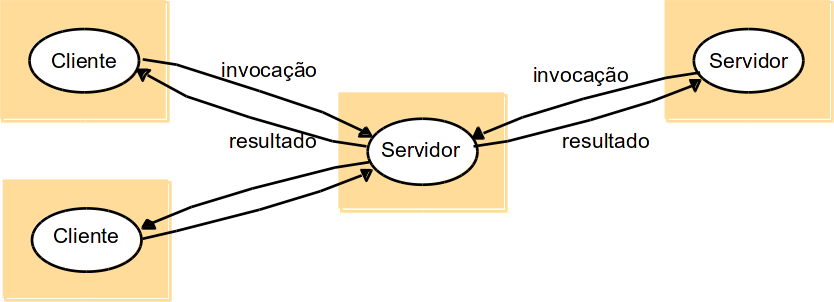
\includegraphics[scale=0.4]{cs2}%% Dimensões e localização
%     \fonte{Adaptado de \citeonline[p.~42]{Coulouris2013}}%% Fonte
%     \addcontentsline{loge}{figure}{\protect\numberline{\thefigure}Exemplo de figura criada a partir de um arquivo.}
% \end{figure}

% Utilizando o pacote \textit{subfig} é possível adicionar figuras lado a lado, como pode ser observado na \autoref{fig:exemplo3}.

% \begin{figure}[htb]
%     \caption{Telas de cadastro de Paciente: (a) Cadastro Paciente, (b) Cadastro Paciente 2} 
% 	\label{fig:exemplo3}
% 	\centering
% 	\subfloat[Cadastro Paciente]{
% 		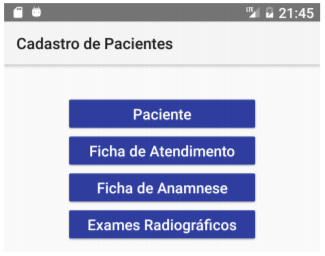
\includegraphics[scale=0.7]{cadastro-paciente}
% 	}\hspace{0.15cm} 
% 	\subfloat[Cadastro Paciente 2]{
% 		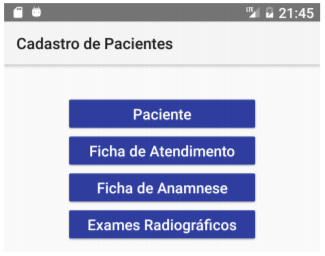
\includegraphics[scale=0.7]{cadastro-paciente}
% 	}	
% 	\fonte{}
%     %\addcontentsline{loge}{figure}{\protect\numberline{\thefigure}Telas de cadastro de Paciente: (a) Cadastro Paciente, (b) Cadastro Paciente 2.}
% \end{figure}

% Este modelo vem com o ambiente \texttt{quadro} e impressão de Lista de quadros configurados por padrão.  Este parágrafo apresenta como referenciar o quadro no texto, requisito obrigatório da \gls{abnt}. Primeira opção, utilizando \texttt{autoref}: Ver o \autoref{quad:exemplo1}. Segunda opção, utilizando  \texttt{ref}: Ver o Quadro \ref{quad:exemplo1}.

% \begin{tabframed}[htb]%% Ambiente tabframed
% %\captionsetup{width=0.5\textwidth}%% Largura da legenda
% \caption{Materiais utilizados no desenvolvimento do sistema}%% Legenda
% \label{quad:exemplo1}%% Rótulo
% \renewcommand{\arraystretch}{1.5}
% \begin{tabular}{|l|l|l|l|l}
% \cline{1-4}
% \textbf{Ferramenta/Tecnologia} & \textbf{Versão} & \textbf{Disponível em} & \textbf{Finalidade} \\ \cline{1-4}
%  Teste & 1.0  & https:/teste.org & Biblioteca de Teste & \\ \cline{1-4}  
%  Teste & 1.0  & https:/teste.org & Biblioteca de Teste & \\ \cline{1-4}
%  Teste & 1.0  & https:/teste.org & Biblioteca de Teste & \\ \cline{1-4}
%  Teste & 1.0  & https:/teste.org & Biblioteca de Teste & \\ \cline{1-4}
% \end{tabular}
% \fonte{}%% Fonte
% \addcontentsline{loge}{tabframed}{\protect\numberline{\thetabframed}Materiais utilizados no desenvolvimento do sistema.}
% \end{tabframed}


% Também é possível citar tabelas no texto. Primeira opção, utilizando \texttt{autoref}: Ver o \autoref{tab:exemplo1}. Segunda opção, utilizando  \texttt{ref}: Ver a Tabela \ref{tab:exemplo1}.

% \begin{table}[htb]
% % Luiz - O texto do caption da tabela/quadro deve ser do tamanho da tabela, então utilize a linha a seguir para conseguir esse efeito
% \captionsetup{width=0.83\textwidth}
% \centering
% \caption{\label{tab:exemplo1}Exemplo de tabela com uma legenda contendo um texto longo}
% \begin{tabular}{cccc}
% 	\hline
% 	\textbf{Pessoa} & \textbf{Idade} & \textbf{Peso} & \textbf{Altura} \\ \hline
% 	Marcos & 26    & 68   & 178    \\ 
% 	Ivone  & 22    & 57   & 162    \\ 
% 	...    & ...   & ...  & ...    \\ 
% 	Sueli  & 40    & 65   & 153    \\ \hline
% \end{tabular}
% \fonte{}
% \end{table}

% A \autoref{tab:exemplo2} também pode ser citada no texto.

% \begin{table}[htb]%% Ambiente table
% \caption{Segundo exemplo de tabela com uma legenda contendo um texto muito longo que pode ocupar mais de uma linha}%% Legenda
% \label{tab:exemplo2}%% Rótulo
% \begin{tabularx}{\textwidth}{@{\extracolsep{\fill}}llll}%% Ambiente tabularx
% \toprule
% $\bsym{L}$ & $\bsym{L^2}$ & $\bsym{L^3}$ & $\bsym{L^4}$ \\
% \SI{}{[m]} & \SI{}{[m^2]} & \SI{}{[m^3]} & \SI{}{[m^4]} \\ \midrule
% 1          & 1            & 1            & 1            \\
% 2          & 4            & 8            & 16           \\
% 3          & 9            & 27           & 81           \\
% 4          & 16           & 64           & 256          \\
% 5          & 25           & 125          & 625          \\ \bottomrule
% \end{tabularx}
% \fonte{}%% Fonte
% \end{table}

% A \autoref{tab:exemplo3} é um exemplo de tabela que ocupa mais de uma página e que foi construída pelo \gls{latex}\index{LaTeX@\latex} utilizando o pacote \texttt{longtable}.

% \begin{longtable}{@{\extracolsep{\fill}}lll}%% Ambiente longtable
% \caption{Possíveis tríplices para grade altamente variável\label{tab:exemplo3}} \\%% Legenda e rótulo
% \toprule
% \textbf{Tempo (s)} & \textbf{Tríplice escolhida} & \textbf{Outras possíveis tríplices} \\
% \midrule
% \endfirsthead%% Encerra cabeçalho da primeira página
% \caption[]{Possíveis tríplices para grade altamente variável} \\%% Legenda
% \multicolumn{3}{r}{\textbf{(continuação)}} \\
% \toprule
% \textbf{Tempo (s)} & \textbf{Tríplice escolhida} & \textbf{Outras possíveis tríplices} \\
% \midrule
% \endhead%% Encerra cabeçalho das demais páginas
% \midrule
% \multicolumn{3}{r}{\textbf{(continua)}} \\
% \endfoot%% Encerra rodapé das demais páginas
% \bottomrule
% \\[-0.5\linha]
% \caption*{\nomefonte: Adaptado de \citeonline[p.~42]{Smallen2014}} \\
% \endlastfoot%% Encerra rodapé da última página
% 0      & (1, 11, 13725) & (1, 12, 10980), (1, 13, 8235), (2, 2, 0), (3, 1, 0) \\
% 2745   & (1, 12, 10980) & (1, 13, 8235), (2, 2, 0), (2, 3, 0), (3, 1, 0)      \\
% 5490   & (1, 12, 13725) & (2, 2, 2745), (2, 3, 0), (3, 1, 0)                  \\
% 8235   & (1, 12, 16470) & (1, 13, 13725), (2, 2, 2745), (2, 3, 0), (3, 1, 0)  \\
% 10980  & (1, 12, 16470) & (1, 13, 13725), (2, 2, 2745), (2, 3, 0), (3, 1, 0)  \\
% 13725  & (1, 12, 16470) & (1, 13, 13725), (2, 2, 2745), (2, 3, 0), (3, 1, 0)  \\
% 16470  & (1, 13, 16470) & (2, 2, 2745), (2, 3, 0), (3, 1, 0)                  \\
% 19215  & (1, 12, 16470) & (1, 13, 13725), (2, 2, 2745), (2, 3, 0), (3, 1, 0)  \\
% 21960  & (1, 12, 16470) & (1, 13, 13725), (2, 2, 2745), (2, 3, 0), (3, 1, 0)  \\
% 24705  & (1, 12, 16470) & (1, 13, 13725), (2, 2, 2745), (2, 3, 0), (3, 1, 0)  \\
% 27450  & (1, 12, 16470) & (1, 13, 13725), (2, 2, 2745), (2, 3, 0), (3, 1, 0)  \\
% 30195  & (2, 2, 2745)   & (2, 3, 0), (3, 1, 0)                                \\
% 32940  & (1, 13, 16470) & (2, 2, 2745), (2, 3, 0), (3, 1, 0)                  \\
% 35685  & (1, 13, 13725) & (2, 2, 2745), (2, 3, 0), (3, 1, 0)                  \\
% 38430  & (1, 13, 10980) & (2, 2, 2745), (2, 3, 0), (3, 1, 0)                  \\
% 41175  & (1, 12, 13725) & (1, 13, 10980), (2, 2, 2745), (2, 3, 0), (3, 1, 0)  \\
% 43920  & (1, 13, 10980) & (2, 2, 2745), (2, 3, 0), (3, 1, 0)                  \\
% 46665  & (2, 2, 2745)   & (2, 3, 0), (3, 1, 0)                                \\
% 49410  & (2, 2, 2745)   & (2, 3, 0), (3, 1, 0)                                \\
% 52155  & (1, 12, 16470) & (1, 13, 13725), (2, 2, 2745), (2, 3, 0), (3, 1, 0)  \\
% 54900  & (1, 13, 13725) & (2, 2, 2745), (2, 3, 0), (3, 1, 0)                  \\
% 57645  & (1, 13, 13725) & (2, 2, 2745), (2, 3, 0), (3, 1, 0)                  \\
% 60390  & (1, 12, 13725) & (2, 2, 2745), (2, 3, 0), (3, 1, 0)                  \\
% 63135  & (1, 13, 16470) & (2, 2, 2745), (2, 3, 0), (3, 1, 0)                  \\
% 65880  & (1, 13, 16470) & (2, 2, 2745), (2, 3, 0), (3, 1, 0)                  \\
% 68625  & (2, 2, 2745)   & (2, 3, 0), (3, 1, 0)                                \\
% 71370  & (1, 13, 13725) & (2, 2, 2745), (2, 3, 0), (3, 1, 0)                  \\
% 74115  & (1, 12, 13725) & (2, 2, 2745), (2, 3, 0), (3, 1, 0)                  \\
% 76860  & (1, 13, 13725) & (2, 2, 2745), (2, 3, 0), (3, 1, 0)                  \\
% 79605  & (1, 13, 13725) & (2, 2, 2745), (2, 3, 0), (3, 1, 0)                  \\
% 82350  & (1, 12, 13725) & (2, 2, 2745), (2, 3, 0), (3, 1, 0)                  \\
% 85095  & (1, 12, 13725) & (1, 13, 10980), (2, 2, 2745), (2, 3, 0), (3, 1, 0)  \\
% 87840  & (1, 13, 16470) & (2, 2, 2745), (2, 3, 0), (3, 1, 0)                  \\
% 90585  & (1, 13, 16470) & (2, 2, 2745), (2, 3, 0), (3, 1, 0)                  \\
% 93330  & (1, 13, 13725) & (2, 2, 2745), (2, 3, 0), (3, 1, 0)                  \\
% 96075  & (1, 13, 16470) & (2, 2, 2745), (2, 3, 0), (3, 1, 0)                  \\
% 98820  & (1, 13, 16470) & (2, 2, 2745), (2, 3, 0), (3, 1, 0)                  \\
% 101565 & (1, 13, 13725) & (2, 2, 2745), (2, 3, 0), (3, 1, 0)                  \\
% 104310 & (1, 13, 16470) & (2, 2, 2745), (2, 3, 0), (3, 1, 0)                  \\
% 107055 & (1, 13, 13725) & (2, 2, 2745), (2, 3, 0), (3, 1, 0)                  \\
% 109800 & (1, 13, 13725) & (2, 2, 2745), (2, 3, 0), (3, 1, 0)                  \\
% 112545 & (1, 12, 16470) & (1, 13, 13725), (2, 2, 2745), (2, 3, 0), (3, 1, 0)  \\
% 115290 & (1, 13, 16470) & (2, 2, 2745), (2, 3, 0), (3, 1, 0)                  \\
% 118035 & (1, 13, 13725) & (2, 2, 2745), (2, 3, 0), (3, 1, 0)                  \\
% 120780 & (1, 13, 16470) & (2, 2, 2745), (2, 3, 0), (3, 1, 0)                  \\
% 123525 & (1, 13, 13725) & (2, 2, 2745), (2, 3, 0), (3, 1, 0)                  \\
% 126270 & (1, 12, 16470) & (1, 13, 13725), (2, 2, 2745), (2, 3, 0), (3, 1, 0)  \\
% 129015 & (2, 2, 2745)   & (2, 3, 0), (3, 1, 0)                                \\
% 131760 & (2, 2, 2745)   & (2, 3, 0), (3, 1, 0)                                \\
% 134505 & (1, 13, 16470) & (2, 2, 2745), (2, 3, 0), (3, 1, 0)                  \\
% 137250 & (1, 13, 13725) & (2, 2, 2745), (2, 3, 0), (3, 1, 0)                  \\
% 139995 & (2, 2, 2745)   & (2, 3, 0), (3, 1, 0)                                \\
% 142740 & (2, 2, 2745)   & (2, 3, 0), (3, 1, 0)                                \\
% 145485 & (1, 12, 16470) & (1, 13, 13725), (2, 2, 2745), (2, 3, 0), (3, 1, 0)  \\
% 148230 & (2, 2, 2745)   & (2, 3, 0), (3, 1, 0)                                \\
% 150975 & (1, 13, 16470) & (2, 2, 2745), (2, 3, 0), (3, 1, 0)                  \\
% 153720 & (1, 12, 13725) & (2, 2, 2745), (2, 3, 0), (3, 1, 0)                  \\
% 156465 & (1, 13, 13725) & (2, 2, 2745), (2, 3, 0), (3, 1, 0)                  \\
% 159210 & (1, 13, 13725) & (2, 2, 2745), (2, 3, 0), (3, 1, 0)                  \\
% 161955 & (1, 13, 16470) & (2, 2, 2745), (2, 3, 0), (3, 1, 0)                  \\
% 164700 & (1, 13, 13725) & (2, 2, 2745), (2, 3, 0), (3, 1, 0)                  \\
% \end{longtable}


% \subsection{Códigos fonte e algoritmos}\label{subsec:algoritimos}

% Os algoritmos podem ser utilizados para explicar uma determinada rotina desenvolvida. Conforme pode ser observado no \autoref{alg:exemplo1}.

% \begin{algorithm}[htb]%% Ambiente algorithm
% \caption{Algoritmo de exemplo}%% Legenda
% \label{alg:exemplo1}%% Rótulo
% \hrule
% \begin{algorithmic}[1]%% Ambiente algorithmic
% \ENSURE $A, B$
% \STATE $C = A + B$
% \IF{$C < 10$}
% \STATE $C = 2 \ C$
% \ELSE
% \STATE $C = 0,5 \ C$
% \ENDIF
% \PRINT $A, B, C$
% \end{algorithmic}
% \hrule
% \fonte{}%% Fonte
% \end{algorithm}

% \lipsum[1]

% \lipsum[1]

% Na \autoref{code:exemplo1} pode ser visualizado um exemplo de código fonte.

% \begin{sourcecode}[htb]
% \caption{\label{code:exemplo1}Exemplo de código}
% \begin{lstlisting}[frame=single, language=Java]
% @Entity
% public class Foo {
 
%     @Id
%     @GeneratedValue(strategy = GenerationType.IDENTITY)
%     private Long id;
 
%     private String name;
%     // constructor, getters and setters
% }
% \end{lstlisting}
% \fonte{}
% \end{sourcecode}

%% Comente para remover este item

%% Capítulo
%%%% CAPÍTULO 5 - CONCLUSÕES E PERSPECTIVAS
%%
\chapter{Conclusão (ou considerações finais)}\label{cap:conclusoeseperspectivas}

Parte final do texto, na qual se apresentam as conclusões do trabalho acadêmico, usualmente denominada Considerações Finais. Pode ser usada outra denominação similar que indique a conclusão do trabalho.
%% Comente para remover este item

%% Capítulo
%\include{./capitulos/cap-trabalhos-relacionados}%% Comente para remover este item

%% Capítulo
%\include{./capitulos/cap-proposta}%% Comente para remover este item

%% Capítulo
%\include{./capitulos/cap-metodologia}%% Comente para remover este item

%% Capítulo
%\include{./capitulos/cap-experimentos-resultados}%% Comente para remover este item

%% Capítulo - esse capítulo contém exemplos para melhor uso do modelo Latex
%% Na versão final do TCC esse capítulo deve ser removido utilizando o sinal %
%\include{./capitulos/cap-exemplo}%% Comente para remover este item

%% Parte
% \part{Conclusão}%% Comente para remover este item

%% Capítulo
%%%%% CAPÍTULO 5 - CONCLUSÕES E PERSPECTIVAS
%%
\chapter{Conclusão (ou considerações finais)}\label{cap:conclusoeseperspectivas}

Parte final do texto, na qual se apresentam as conclusões do trabalho acadêmico, usualmente denominada Considerações Finais. Pode ser usada outra denominação similar que indique a conclusão do trabalho.
%% Comente para remover este item

%% Capítulos após este comando criam marcadores do pdf na raiz
% \phantompart%% Comente para remover este item


%% Formatação de páginas de elementos pós-textuais
\postextual%% Não comente esta linha

%% Arquivos de referências
\arquivosdereferencias{%% Arquivos bibtex sem a extensão .bib e separados por vírgula - Não comente esta linha
  %./PosTexto/exemplos-referencias,%% Arquivo de referências - Comente para remover este item
  main%% Arquivo de referências - Comente para remover este item
}%% Não comente esta linha

%% Glossário
%\incluirglossario %% Comente para remover este item

\renewcommand{\ABNTEXchapterfont}{\bfseries}
\renewcommand{\ABNTEXchapterfontsize}{\normalsize}
\renewcommand{\thechapter}{\Alph{chapter}} % Letra ao invés de número
\renewcommand{\chaptername}{Apêndice} % Muda a palavra "Capítulo" para "Apêndice"

%% Arquivos de apêndices
\begin{arquivosdeapendices}%% Os arquivos de apêndices devem se incluídos neste ambiente - Não comente esta linha
%  \partapendices%% Página de início dos apêndices - adiciona uma página com o título Apêndices
%   %% Capítulo de exemplo
%\begin{apendicesenv}
   %%%% APÊNDICE A
    \cleardoublepage
    \thispagestyle{empty}
    \refstepcounter{chapter} % incrementa o contador
    %\chapter*{Apêndice~\thechapter\\[1ex]Questionário de pesquisa}   
    \vspace*{\fill}
    \begin{center}
        {\bfseries APÊNDICE~\thechapter{ -- }Questionário de pesquisa}
    \end{center}
    \vspace*{\fill}
    \addcontentsline{toc}{chapter}{APÊNDICE~\thechapter{ -- } Questionário de pesquisa}

%\chapter{Questionário de pesquisa}\label{cap:apendicea}
\newpage
\centerline{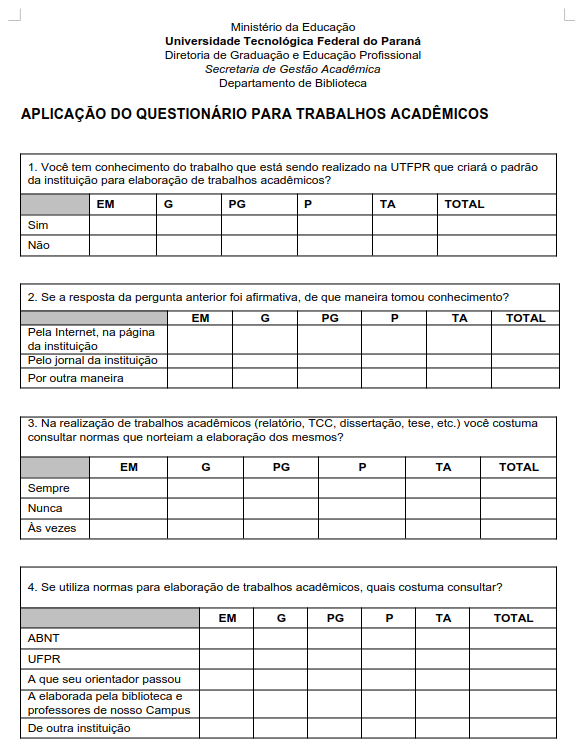
\includegraphics[width=\textwidth]{./PosTexto/Ilustracoes/questionario}}%% Imagem (Dimensões e localização)%% Apêndice - Comente para remover este item
   
%\chapter{Roteiro da entrevista}\label{cap:apendiceb}
%\apendices

    \cleardoublepage
    \thispagestyle{empty}
    \refstepcounter{chapter} % incrementa o contador
    %\chapter*{Apêndice~\thechapter\\[1ex]Questionário de pesquisa}   
    \vspace*{\fill}
    \begin{center}
        {\bfseries APÊNDICE~\thechapter{ -- }Roteiro da entrevista}
    \end{center}
    \vspace*{\fill}
    \addcontentsline{toc}{chapter}{APÊNDICE~\thechapter{ -- } Roteiro da entrevista}

\newpage
\centerline{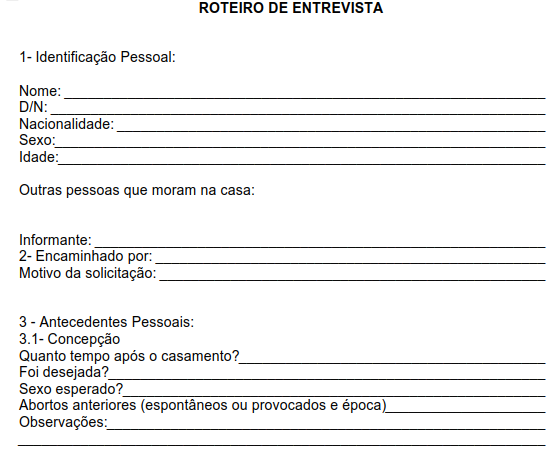
\includegraphics[width=\textwidth]{./PosTexto/Ilustracoes/roteiro}}%% Imagem (Dimensões e localização)%% Apêndice - Comente para remover este item
   
    \cleardoublepage
    \thispagestyle{empty}
    \refstepcounter{chapter} % incrementa o contador
    %\chapter*{Apêndice~\thechapter\\[1ex]Questionário de pesquisa}   
    \vspace*{\fill}
    \begin{center}
        {\bfseries APÊNDICE~\thechapter{ -- }Abreviaturas dos meses do ano}
    \end{center}
    \vspace*{\fill}
    \addcontentsline{toc}{chapter}{APÊNDICE~\thechapter{ -- } Abreviaturas dos meses do ano}
    
%\chapter{Abreviaturas dos meses do ano}\label{cap:apendicec}
\newpage

%\centerline{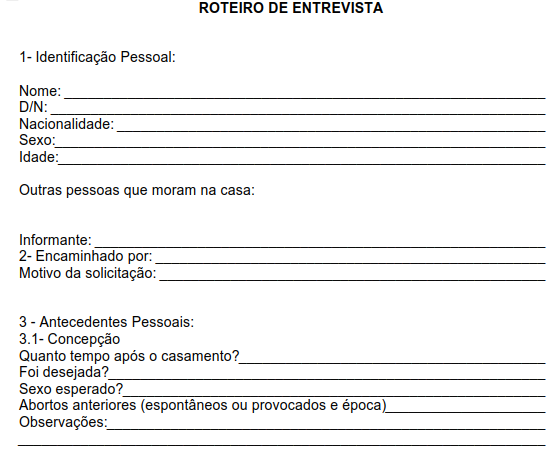
\includegraphics[width=\textwidth]{./PosTexto/Ilustracoes/roteiro}}%% Imagem (Dimensões e localização)

\begin{center}
\textbf{Abreviaturas dos meses do ano}    
\end{center}


\doublespacing{

\begin{tabular}{l l}
Janeiro –  &  jan. \\
Fevereiro –  & fev. \\
Março –  &mar.\\
Abril –   &abr.\\
Maio –  &maio (único não abreviado).\\
Junho –   &jun. \\
Julho –   &jul.\\
Agosto –  &ago.\\
Setembro –  &set.\\
Outubro –  &out.\\
Novembro –  &nov.\\
Dezembro –  &dez.\\
\end{tabular}
}%% Apêndice - Comente para remover este item
%\end{apendicesenv}
\end{arquivosdeapendices}%% Não comente esta linha


% \begin{apendicesenv}%% Ambiente apendicesenv

% %\partapendices
% % \chapter{Ola}

% % \lipsum[55-56]

% \end{apendicesenv}

%% Arquivos de anexos
\begin{arquivosdeanexos}%% Os arquivos de anexos devem se incluídos neste ambiente - Não comente esta linha
  %\partanexos%% Página de início dos anexos - adiciona uma página com o título Anexosm
   %%%% ANEXO A
%%
%% Texto ou documento não elaborado pelo autor, que serve de fundamentação, comprovação e ilustração.

%% Título e rótulo de anexo (rótulos não devem conter caracteres especiais, acentuados ou cedilha)
\anexos
  \cleardoublepage
    \thispagestyle{empty}
    \refstepcounter{chapter} % incrementa o contador
    %\chapter*{Apêndice~\thechapter\\[1ex]Questionário de pesquisa}   
    \vspace*{\fill}
    \begin{center}
        {\bfseries ANEXO~\thechapter{ -- }Lei N\texorpdfstring{.\textsuperscript{o}}{o.} 9.610, de 19 de Fevereiro de 1998}
    \end{center}
    \vspace*{\fill}
    \addcontentsline{toc}{chapter}{ANEXO~\thechapter{ -- }Lei N\texorpdfstring{.\textsuperscript{o}}{o.} 9.610, de 19 de Fevereiro de 1998}

%\chapter{Lei N\texorpdfstring{.\textsuperscript{o}}{o.} 9.610, de 19 de Fevereiro de 1998}\label{cap:anexoa}


\newpage
\centerline{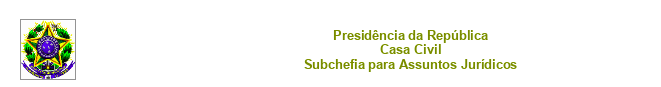
\includegraphics[width=\textwidth]{./PosTexto/Ilustracoes/top.png}}%% Imagem (Dimensões e localização)

\begin{center}
\textbf{LEI Nº 9.610, DE 19 DE FEVEREIRO DE 1998\footnote{Disponível em:\url{http://www.planalto.gov.br/ccivil_03/leis/l9610.htm.}}.}
\end{center}

\hspace{7cm}\parbox{8cm}{\scriptsize{\textcolor{red}{Altera, atualiza e consolida a legislação sobre direitos autorais e dá outras providências.}}}
\vspace{0.3cm}

\textbf{O PRESIDENTE DA REPÚBLICA} Faço saber que o Congresso Nacional decreta e eu sanciono a seguinte Lei:

\begin{center}
Título I - Disposições Preliminares
\end{center}

\scriptsize{
Art. 1º Esta Lei regula os direitos autorais, entendendo-se sob esta denominação os direitos de autor e os que lhes são conexos. 

Art. 2º Os estrangeiros domiciliados no exterior gozarão da proteção assegurada nos acordos, convenções e tratados em vigor no Brasil.

Parágrafo único. Aplica-se o disposto nesta Lei aos nacionais ou pessoas domiciliadas em país que assegure aos brasileiros ou pessoas domiciliadas no Brasil a reciprocidade na proteção aos direitos autorais ou equivalentes.

Art. 3º Os direitos autorais reputam-se, para os efeitos legais, bens móveis.

Art. 4º Interpretam-se restritivamente os negócios jurídicos sobre os direitos autorais.

Art. 5º Para os efeitos desta Lei, considera-se:

I - publicação - o oferecimento de obra literária, artística ou científica ao conhecimento do público, com o consentimento do autor, ou de qualquer outro titular de direito de autor, por qualquer forma ou processo;

II - transmissão ou emissão - a difusão de sons ou de sons e imagens, por meio de ondas radioelétricas; sinais de satélite; fio, cabo ou outro condutor; meios óticos ou qualquer outro processo eletromagnético; 

III - retransmissão - a emissão simultânea da transmissão de uma empresa por outra;

IV - distribuição - a colocação à disposição do público do original ou cópia de obras literárias, artísticas ou científicas, interpretações ou execuções fixadas e fonogramas, mediante a venda, locação ou qualquer outra forma de transferência de propriedade ou posse;

V - comunicação ao público - ato mediante o qual a obra é colocada ao alcance do público, por qualquer meio ou procedimento e que não consista na distribuição de exemplares;

VI - reprodução - a cópia de um ou vários exemplares de uma obra literária, artística ou científica ou de um fonograma, de qualquer forma tangível, incluindo qualquer armazenamento permanente ou temporário por meios eletrônicos ou qualquer outro meio de fixação que venha a ser desenvolvido;

VII - contrafação - a reprodução não autorizada;

VIII - obra: 

a) em co-autoria - quando é criada em comum, por dois ou mais autores;

b) anônima - quando não se indica o nome do autor, por sua vontade ou por ser desconhecido;

c) pseudônima - quando o autor se oculta sob nome suposto;

d) inédita - a que não haja sido objeto de publicação;

e) póstuma - a que se publique após a morte do autor;

f) originária - a criação primígena;

g) derivada - a que, constituindo criação intelectual nova, resulta da transformação de obra originária;

h) coletiva - a criada por iniciativa, organização e responsabilidade de uma pessoa física ou jurídica, que a publica sob seu nome ou marca e que é constituída pela participação de diferentes autores, cujas contribuições se fundem numa criação autônoma;

i) audiovisual - a que resulta da fixação de imagens com ou sem som, que tenha a finalidade de criar, por meio de sua reprodução, a impressão de movimento, independentemente dos processos de sua captação, do suporte usado inicial ou posteriormente para fixá-lo, bem como dos meios utilizados para sua veiculação;

IX - fonograma - toda fixação de sons de uma execução ou interpretação ou de outros sons, ou de uma representação de sons que não seja uma fixação incluída em uma obra audiovisual;

X - editor - a pessoa física ou jurídica à qual se atribui o direito exclusivo de reprodução da obra e o dever de divulgá-la, nos limites previstos no contrato de edição; 

XI - produtor - a pessoa física ou jurídica que toma a iniciativa e tem a responsabilidade econômica da primeira fixação do fonograma ou da obra audiovisual, qualquer que seja a natureza do suporte utilizado;

XII - radiodifusão - a transmissão sem fio, inclusive por satélites, de sons ou imagens e sons ou das representações desses, para recepção ao público e a transmissão de sinais codificados, quando os meios de decodificação sejam oferecidos ao público pelo organismo de radiodifusão ou com seu consentimento;

XIII - artistas intérpretes ou executantes - todos os atores, cantores, músicos, bailarinos ou outras pessoas que representem um papel, cantem, recitem, declamem, interpretem ou executem em qualquer forma obras literárias ou artísticas ou expressões do folclore.

Art. 6º Não serão de domínio da União, dos Estados, do Distrito Federal ou dos Municípios as obras por eles simplesmente subvencionadas.
}

%% Anexo - Comente para remover este item
\end{arquivosdeanexos}%% Não comente esta linha

%% Índice - Adiciona um índice remissivo.
%\incluirindice%% Comente para remover este item

%% Fim do documento
\end{document}%% Não comente esta linha
